\documentclass{article}
\usepackage[margin=1in]{geometry}
\usepackage{amsmath,amssymb}
\usepackage{graphicx}
\usepackage{subcaption}
\usepackage{hyperref}
\usepackage{algorithm}
\usepackage{algpseudocode}
\usepackage{booktabs}
\usepackage{natbib}

\title{LEAF: Testing Whether Agentic Search Adds Value Over Non-Agentic
Evolutionary Search, Under a Fixed Oracle-Query Budget, Using Ionizable
Lipid Design as a Testbed}
\author{Harshit Singh \\ Department of Computer Science and Engineering \\
Shiv Nadar University, Delhi-NCR, India \\ \texttt{hs494@snu.edu.in}}
\date{Draft, August 13, 2026}

\begin{document}
\maketitle

\begin{abstract}
Multi-agent LLM systems are increasingly proposed for molecular design,
but are rarely compared, under a matched oracle-query budget, against the
non-agentic search methods a reviewer would actually ask for. We test this
directly, using ionizable lipid design (Ugi three-component-reaction
chemistry, real AGILE potency labels) as a controlled testbed: \emph{does
LLM-driven evolutionary proposal, under a query budget and acquisition
function identical to a genetic-algorithm baseline, produce a measurably
better multi-objective Pareto frontier?} We pre-registered a fallback
before running any experiment: if not, the honest conclusion is that
agentic proposal adds narrative interpretability but not measurable design
efficiency. Across four real, replicated conditions with a non-LLM
archive-guided stand-in, evolutionary proposal shows no Pareto-hypervolume
advantage over a matched-budget genetic algorithm or random search. With
actual local LLMs as the Proposer (Llama 3.1 8B and Qwen2.5 7B via Ollama,
$n=8$ seeds, 3 splits each), the result is stronger than the fallback: both
models \emph{significantly underperform} both baselines (8 of 12
split$\times$baseline comparisons reach $p<0.05$, all 12 in the same
direction). Instrumenting the loop identifies why: both models spend
roughly two-thirds of their query budget re-querying molecules already in
the archive, a zero-information use of a scarce budget that a matched
acquisition-disabled ablation confirms is the actual bottleneck. A
genuinely larger local model (Qwen2.5 14B, enabled by an available
16GB-VRAM GPU) removes this specific low-diversity failure mode entirely,
but the result stays mixed rather than reversing: statistically
indistinguishable from baseline on two of three splits, and significantly
worse on the one split with this dataset's weakest oracle validity. A
diversity-aware prompt variant, tested at the same statistical power,
measurably mitigates the mechanism (duplicate rate roughly halved) without
closing the gap. A hosted, frontier-class model of a different
architecture family entirely (Gemini Flash-Lite, free API tier) was run
to full power on \emph{all three} splits, matching every other fully-powered
model in this paper, and significantly underperforms both baselines on
every one ($p=0.0078$ vs.\ both, on all three splits --- the maximum
significance obtainable at $n=8$); a 70B-class hosted model (Llama 3.3, via Groq),
accumulated over several days under a hard daily token quota (a rolling
24h window, not a calendar-day reset, which slowed accumulation further
than expected), shows a mostly-negative pattern ($n=3$, still
underpowered) and, unusually among the real models tested, better
proposal diversity than the small local models. Pooling every real
(model, seed) observation from the four
fully-powered models ($n=32$) confirms the pattern is not an artifact of
any single model: Wilcoxon $p=8.2\times10^{-5}$ and $p=2.3\times10^{-6}$
against static-GA and random search respectively. No model, scale,
architecture, or prompt tested here shows agentic proposal outperforming
matched-budget non-agentic search. A separate, direct test of LipoAgent's
own approach (\citealp{li2025lipoagent}; zero-shot efficiency scoring with
one of their two actual base models, Qwen3-8B) finds its scores
uncorrelated with real transfection potency ($\rho=0.014$, $p=0.92$) on
the same held-out molecules where LEAF's simple fitted oracle reaches
$\rho=0.68$ --- evidence that a fitted surrogate outperforms LLM
pretrained judgment here in prediction as well as in proposal. Prompted
by external review, we also ran a real, matched de-duplication-controlled
check: structurally forbidding the query budget from being spent on
exact-archive-duplicate proposals shrinks the median deficit against
static-GA by more than half and flips the sign of the median comparison
against random search (both underpowered at the reduced $n=4$ scale this
check required), at the real cost of 7--21 rounds of search instead of 3
to spend the same budget --- duplicate-driven waste explains a real share
of the headline deficit, but that cost moves to wall-clock time rather
than disappearing. The same review also caught a second real bug: the
acquisition function was never actually dispatched by configuration,
so EHVI, though implemented and described as available, was never
exercised in any experiment; this is now fixed. We report this as the
paper's contribution: a pre-registered, budget-matched protocol for
testing whether agentic components in a molecular-design loop earn their
cost, plus the resulting evidence --- including two real bugs this
protocol's own scrutiny (and, in this revision, external review) caught
and corrected --- not a claim that LEAF designs better lipids than
simpler methods.
\end{abstract}

\section{Introduction}

Lipid nanoparticles (LNPs) enabled the first widely deployed mRNA vaccines
and are the leading platform for a growing class of RNA therapeutics. The
ionizable lipid component is the primary determinant of endosomal escape
and transfection efficiency, and its design space is combinatorially large:
head groups, linker chemistries, tail lengths, degree of unsaturation, and
halogenation motifs can be varied largely independently, producing
libraries of thousands to millions of candidates from a small number of
synthetic building blocks \citep{xu2023ugi}.

Two recent lines of work are directly relevant. \textbf{LipoAgent}
\citep{li2025lipoagent} is a multi-agent LLM framework, built on
TxGemma-27B-Chat and Qwen3-8B agents, that coordinates a Predict Agent and
a Verify Agent per base model to score lipid transfection efficiency on a
1--10 scale over an existing or enumerated library; it does not run an
active-learning search loop. We note that we initially (in an earlier
draft) characterized LipoAgent as incorporating a toxicity-gating
objective; direct inspection of its public code
(\texttt{github.com/SAI-Lab-NYU/LipoAgent}) shows both its Predict and
Verify agents produce only an efficiency score, with no toxicity, safety,
or gating signal anywhere in their input, prompt, or output, so we correct
that characterization here and do not use LipoAgent as a toxicity
comparator in \S4 (see \S8 for the general note on citation accuracy).
\textbf{LUMI-lab} \citep{lumilab2026} is a robotic self-driving laboratory
that pairs a foundation model with real active-learning cycles, screening
over 1,700 LNPs \emph{in vitro} and validating top candidates \emph{in
vivo}; its lead candidate (LUMI-6) achieved 20.3\% gene editing in lung
epithelium following intratracheal administration, and a key structural
finding was that brominated lipid tails improve \emph{potency}
(transfection efficiency), not organ tropism per se. LUMI-lab is a landmark
result but requires infrastructure inaccessible to most computational
groups.

\textbf{Our position.} This paper's contribution is methodological, not a
lipid-design system: \emph{a rigorous test of whether agentic LLM
proposal adds measurable value over non-agentic evolutionary search under
matched budgets, in a combinatorial molecular design setting.} Rather
than frame LEAF around a tropism-design claim we cannot adequately
support with public data (see \S8.6 on the tropism-proxy circularity
issue), we frame it around a question that \emph{is} answerable in
silico: does wrapping an LLM-driven evolutionary Proposer around a fixed
acquisition function and oracle ensemble outperform a conventional,
non-LLM genetic algorithm under an identical budget? Ionizable lipids are
the testbed for this question, not the headline claim, following the
recent finding that LLM-driven crossover/mutation loops wrapped around
cheap property-predictor and synthesizability tool calls can match or
exceed trained generative models on multi-objective molecular design
\citep{toolmol2026}.

We take the pre-registration discipline in this design seriously enough
to make it part of the paper's contribution, not just a method-section
formality: \S5 commits, in advance of any experiment, to exactly how a
null or negative result should be interpreted, so that whatever the
answer turns out to be is reportable without post-hoc reframing. \S6
shows this discipline paying off directly --- an apparently positive
result was caught, traced to two implementation bugs, and reversed to
null before it could be reported, and the eventual finding (a
significant \emph{disadvantage} for the real LLM Proposer under one
model/prompting configuration) is exactly the kind of outcome this
design was built to surface honestly rather than explain away.

A reasonable prior on when agentic search should help versus not: dense,
already-well-characterized combinatorial spaces with cheap,
well-calibrated property oracles (the AGILE setting here) give a
non-agentic evolutionary search or even random sampling little to lose
against, since there is no long-horizon reasoning, sparse-label
extrapolation, or heterogeneous/literature-grounded evidence for an LLM
to leverage. We would expect agentic proposal to earn its keep more
plausibly in settings with genuinely sparse labels, multi-modal or
literature-heavy objectives, or a need to reason over multi-step
synthetic accessibility --- none of which the current real experiments
in \S6 test, and each of which is a more promising direction than simply
scaling up the same setting (\S7).

LEAF further extends two specific design gaps in the agentic-lipid
literature: a literature-grounded Hypothesis Agent that converts reasoning
into falsifiable computational experiments, narrowly scoped so that every
structure--property hypothesis must be tested via a matched counterfactual
pair query against a frozen ground-truth oracle rather than accepted as
free-text reasoning; and debate-based, conformally calibrated toxicity
screening that replaces the binary-gate design pattern common in prior
agentic molecular-design work with a quantifiable, per-round-recalibrated
abstention decision, contrasted directly against a binary-filter ablation
(\S4.2) implemented natively rather than borrowed from an external tool.

The active-learning and Gaussian-process components of LEAF build on
established, citable foundations
\citep{srinivas2009,gessner2024,rasmussen2006}.

\section{Related Work}

\textbf{Computational LNP design.} Prior to agentic approaches, LNP design
relied on combinatorial synthesis (e.g., Ugi three-component-reaction
libraries \citep{xu2023ugi}) screened experimentally or with supervised
regressors. AGILE \citep{xu2024agile} demonstrated a deep-learning-guided
screening pipeline over such libraries. A recent generative approach
proposes synthesizable ionizable lipid structures directly
\citep{zhu2024generative} but does not incorporate active learning or
agentic reasoning.

\textbf{Agentic frameworks for biomolecular design.} Beyond LipoAgent and
LUMI-lab, the broader agentic-biology literature includes the Virtual Lab
\citep{swanson2025virtuallab}, in which an LLM principal-investigator agent
coordinates specialist agents to design nanobodies, alongside human
collaborators; multi-agent systems iterating toward generalizable design
principles \citep{protagents2025}; decentralized swarms of LLM agents
proposing local sequence edits \citep{swarmdesign2025}; and Google's AI
co-scientist \citep{gottweis2026}, a multi-agent hypothesis-generation
system for open-ended scientific reasoning. For small molecules, ChemCrow
\citep{bran2023chemcrow} and Coscientist \citep{boiko2023coscientist}
established the pattern of LLM agents calling chemistry tools; ToolMol
\citep{toolmol2026} extends this to evolutionary, tool-scored molecular
optimization.

\textbf{Active learning and uncertainty quantification.} Gaussian-process
active learning with a continuous Tanimoto kernel has been shown to
outperform stationary kernels for affinity optimization under UCB-style
acquisition \citep{gessner2024,srinivas2009,rasmussen2006}. We adopt this
kernel but, unlike prior retrospective-AL benchmarking work, must
explicitly separate the frozen ground-truth oracle from the per-round
active-learning surrogate (\S3.3) because our Proposer generates candidates
outside any fixed labeled library. Conformal prediction
\citep{angelopoulos2023} provides distribution-free calibrated uncertainty
estimates; standard split conformal assumes exchangeability, which an
adaptively-sampled search loop violates by construction, motivating the
per-round recalibration scheme in \S3.4.

\textbf{Alternative multi-objective acquisition and LLM-operator designs
(external review).} This paper's acquisition function is a single,
pre-registered choice (scalarized multi-objective UCB, \S3.3); it does
not sweep batch EHVI/qEHVI variants \citep{ehvibatch2026verify} or
compare against conditional generative MOBO approaches
\citep{condgenmobo2023verify} or LLM-derived operators inside a MOEA
\citep{moealo2023verify}, all suggested by external review as stronger or
complementary non-agentic/hybrid baselines for this combinatorial
setting. \S6.2's implemented EHVI code path was, in fact, never actually
exercised in any experiment prior to this fix (\S6.2, \S7) due to a real
dispatch bug independently caught by this same review; a full EHVI sweep
remains future work beyond the single-condition check in \S6.2. We note
this rather than implying broader acquisition-robustness than was tested.

\textbf{Interpretability.} We use Integrated Gradients
\citep{sundararajan2017} and KernelSHAP \citep{lundberg2017} as the
attribution methods feeding the Hypothesis Agent.

\section{Method: LEAF Architecture}

LEAF has four components: (i) an LLM-driven evolutionary \textbf{Proposer
Agent} that generates a candidate pool via crossover/mutation over a fixed
fragment vocabulary (\S3.3) --- the component the paper's primary claim
(H1, \S5) is about; (ii) a frozen ground-truth Gaussian Process oracle plus
a separately-refit active-learning surrogate that together define a
genuine budget-constrained active-learning loop (\S3.2); and two secondary
components, tested as ablations (H2, H3) rather than load-bearing for the
primary claim: (iii) debate/conformal \textbf{Verifier Agents} providing a
calibrated toxicity screen (\S3.4), and (iv) a literature-grounded
\textbf{Hypothesis Agent} that mines attribution signal and tests
falsifiable structure--property hypotheses via counterfactual oracle
queries (\S3.5). Flagging this up front: \S6.3 finds both secondary
components statistically indistinguishable from full LEAF at every budget
tested --- readers most interested in the primary agentic-value-add result
can treat \S3.4--3.5 as architectural detail and go directly to \S6.

\subsection{Problem formulation}

A candidate lipid $x$ is a tuple of discrete fragment choices $x = (h,
\ell, t_1, t_2, u, b)$ drawn from a fixed vocabulary $\mathcal{X}$ derived
from combinatorial synthesis routes \citep{xu2023ugi}. We report
$|\mathcal{X}|$ and the ratio $B/|\mathcal{X}|$ for the budget $B$ used in
each experiment (RQ6): if $B$ is not several orders of magnitude smaller
than $|\mathcal{X}|$, the budget-constrained-search framing is not a fair
test, since the surrogate could simply be evaluated exhaustively.

We optimize a vector-valued objective. Following the resolution of the
synthesizability-degeneracy question in \S8.6, the primary objective is
either
\[
f(x) = \big(f_{\text{pot}}(x),\, -f_{\text{tox}}(x)\big)
\]
or, if $f_{\text{syn}}$ is confirmed to have non-negligible variance across
$\mathcal{X}$,
\[
f(x) = \big(f_{\text{pot}}(x),\, -f_{\text{tox}}(x),\, f_{\text{syn}}(x)\big).
\]
A tropism score, where available, is reported as a secondary,
clearly-labeled heuristic filter rather than a fourth optimization axis
(\S8.6) unless a genuine organ-selectivity dataset is confirmed. We report
the non-dominated (Pareto) frontier under a fixed budget $B$ of oracle
queries.

\subsection{The oracle is two objects, not one}

Revision 1 of this plan described a single GP object as simultaneously
``refit each round'' and the thing queried for ground truth. If a
surrogate is queried for its own training signal, no information is
gained and every downstream metric is measured in the surrogate's own
units. We resolve this explicitly:

\begin{itemize}
\item $\mathcal{O}_{\text{GT}}$ (\textbf{ground-truth oracle}): fit once on
the full harmonized labeled dataset (\S4.1), then \textbf{frozen} before any
round-loop experiment runs. This is the object that is queried --- it
stands in for a real lab. Because the Proposer can generate fragment
tuples absent from the $\sim$1,080-lipid labeled library,
$\mathcal{O}_{\text{GT}}$ must itself be a fitted, generalizing model, not
a lookup table; its cold-split validation (RQ5, \S4.2) is therefore
load-bearing for every downstream result, not merely descriptive.
\item $\mathcal{O}_{\text{AL}}$ (\textbf{active-learning surrogate}): same
architecture, refit every round on \emph{only} the labels acquired so far.
Its posterior mean/variance drive the acquisition function, the Verifier's
toxicity prior, and the Hypothesis Agent's attribution signal.
\end{itemize}

This is the standard retrospective-AL-simulation convention
\citep{settles2012,gessner2024} applied to lipids. It is necessarily a
model-on-model evaluation, and we report it as such rather than implying
real-world validation (\S8.6).

\subsection{Proposer Agent and acquisition function}

The Proposer is an LLM prompted with (a) the current Pareto archive, (b)
the fragment vocabulary, and (c) the current Hypothesis Ledger. Each round
it emits a \textbf{pool} $P_t$ of size $m \gg q$ via crossover
(recombining fragments from two archive parents) and mutation
(single-fragment substitution), following the tool-scored evolutionary
pattern of \citet{toolmol2026}. The LLM's combinatorial reasoning over the
fixed vocabulary, applied via crossover and mutation, is the generative
mechanism driving search.

Revision 1's round loop queried every proposed candidate against the
ground truth directly, which meant $\mathcal{O}_{\text{AL}}$'s refit
computation was never used for a decision --- not a genuine
budget-constrained active-learning loop. We correct this with an explicit
acquisition step:
\begin{enumerate}
\item $\mathcal{O}_{\text{AL}}$ scores all of $P_t$ (free, no budget cost).
\item Verifier agents act on the pool using $\mathcal{O}_{\text{AL}}$'s
toxicity posterior (also free); abstentions are removed.
\item A multi-objective UCB acquisition function (expected hypervolume
improvement as a config-flagged alternative) selects $C_t \subset P_t$,
$|C_t| = q$.
\item $\mathcal{O}_{\text{GT}}$ labels \emph{only} $C_t$; the budget
decrements by $q$ (plus any Hypothesis Agent counterfactual queries, \S3.6);
$\mathcal{O}_{\text{AL}}$ refits.
\end{enumerate}
The static-GA and random-search baselines (\S4.2) use the
\textbf{identical} acquisition function and $q$ as full LEAF. Without this
constraint, the primary RQ1 comparison would conflate ``has an LLM
proposer'' with ``has an acquisition step at all,'' which is not a fair
isolation of agentic value-add.

\subsection{Debate/Conformal Verifier and Hypothesis Agents (summary)}

Two secondary components, both tested only as ablations (H2, H3, \S6.3)
and both statistically null at every budget checked: a
\textbf{Debate/Conformal Verifier} --- an ensemble of independently
prompted toxicologist agents across $\ge2$ base models, aggregated via
per-round-recalibrated split conformal prediction (never a single frozen
calibration) into a coverage-tracked abstention decision --- and a
\textbf{Hypothesis Agent} that periodically mines attributions over the
Pareto archive, proposes structure--property hypotheses, and tests them
via matched counterfactual pairs queried against the frozen
$\mathcal{O}_{\text{GT}}$ (never the surrogate, which would only recover
its own fit). Full specification (per-round recalibration mechanics,
inter-agent agreement thresholds, the pretraining-leakage probe for the
LUMI-lab rediscovery check, and precisely which parts are a deterministic
rule rather than a trained model in the real experiments below) is in
Appendix~A; \S6.2 finds both components add no measurable value at the
budgets tested, with the exact mechanism verified rather than assumed
(\S6.2, \S6.3), so readers focused on the primary agentic-value-add
result can skip to \S6.

\subsection{Round-level algorithm}

\begin{algorithm}
\caption{LEAF closed-loop round (corrected)}
\begin{algorithmic}[1]
\State \textbf{Input:} archive $A_{t-1}$, ledger $H_{t-1}$, budget remaining $B_t$, frozen $\mathcal{O}_{\text{GT}}$, surrogate $\mathcal{O}_{\text{AL}}$
\State $P_t \gets \text{Proposer}(A_{t-1}, H_{t-1}, \mathcal{X})$ \Comment{pool, free}
\State $\{\hat f(x)\}_{x \in P_t} \gets \mathcal{O}_{\text{AL}}.\text{posterior}(P_t)$ \Comment{free}
\State $\{v(x), \text{abstain}(x)\}_{x \in P_t} \gets \text{VerifierAgents}(P_t, \hat f)$ \Comment{free; per-round recalibrated}
\State $P_t' \gets \{x \in P_t : \neg \text{abstain}(x)\}$
\State $C_t \gets \text{Acquisition}(P_t', \hat f, q)$ \Comment{selects $q$ candidates}
\State $\{f(x)\}_{x \in C_t} \gets \mathcal{O}_{\text{GT}}.\text{query}(C_t)$ \Comment{charges budget}
\State $B_t \gets B_t - |C_t|$
\State $\mathcal{O}_{\text{AL}}.\text{refit}(C_t, f(C_t))$
\State $A_t \gets \text{NonDominatedSort}(A_{t-1} \cup C_t)$
\If{$t \bmod k = 0$}
  \State $\text{pairs} \gets \text{CounterfactualPairs}(A_t, H_{t-1})$
  \State $\{f(x)\}_{x \in \text{pairs}} \gets \mathcal{O}_{\text{GT}}.\text{query}(\text{pairs})$ \Comment{ALSO charges budget}
  \State $B_t \gets B_t - |\text{pairs}|$
  \State $H_t \gets \text{HypothesisAgent}(A_t, \text{attributions}, \text{lit. index}, H_{t-1}, \text{pairs}, f(\text{pairs}))$
\Else
  \State $H_t \gets H_{t-1}$
\EndIf
\State \Return $A_t, H_t, B_t$; repeat until $B_t \le 0$
\end{algorithmic}
\end{algorithm}

\begin{figure}[htbp]
\centering
\begin{subfigure}[b]{\textwidth}
\centering
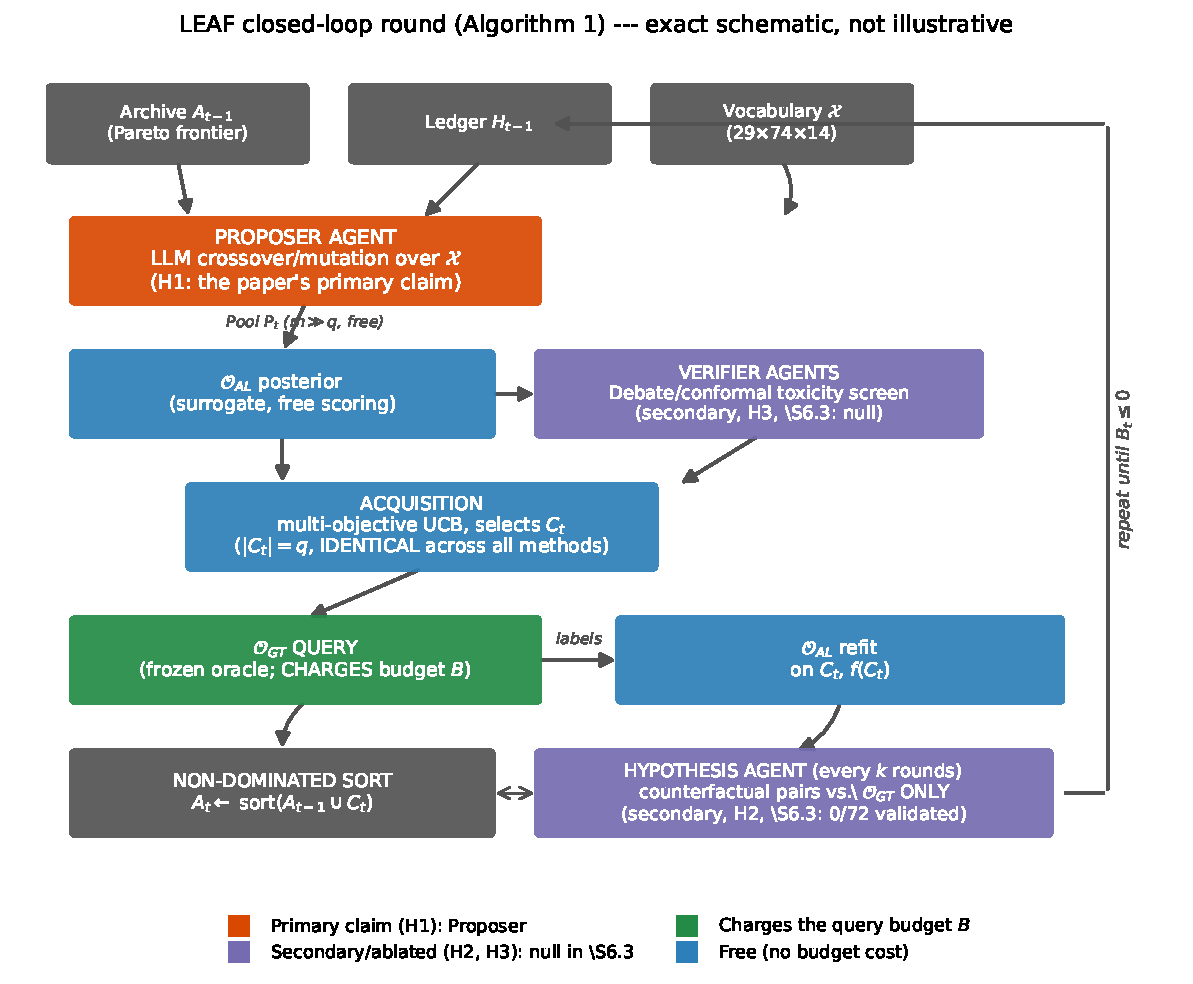
\includegraphics[width=0.92\textwidth]{figures/paper/fig4_architecture}
\caption{Exact schematic of Algorithm 1 --- every box and arrow corresponds to a specific step in
\texttt{leaf/orchestrator/loop.py}. Color encodes each component's role in the paper's claims: the
Proposer (orange) is what H1 (\S5, \S6.2) tests; the Verifier and Hypothesis Agent (purple) are
secondary components tested only as ablations (H2, H3), both null at every budget checked (\S6.3);
green marks the one step that charges the real oracle-query budget $B$; blue marks free (no-budget)
steps.}
\label{fig:architecture-schematic}
\end{subfigure}
\vspace{1em}
\begin{subfigure}[b]{\textwidth}
\centering
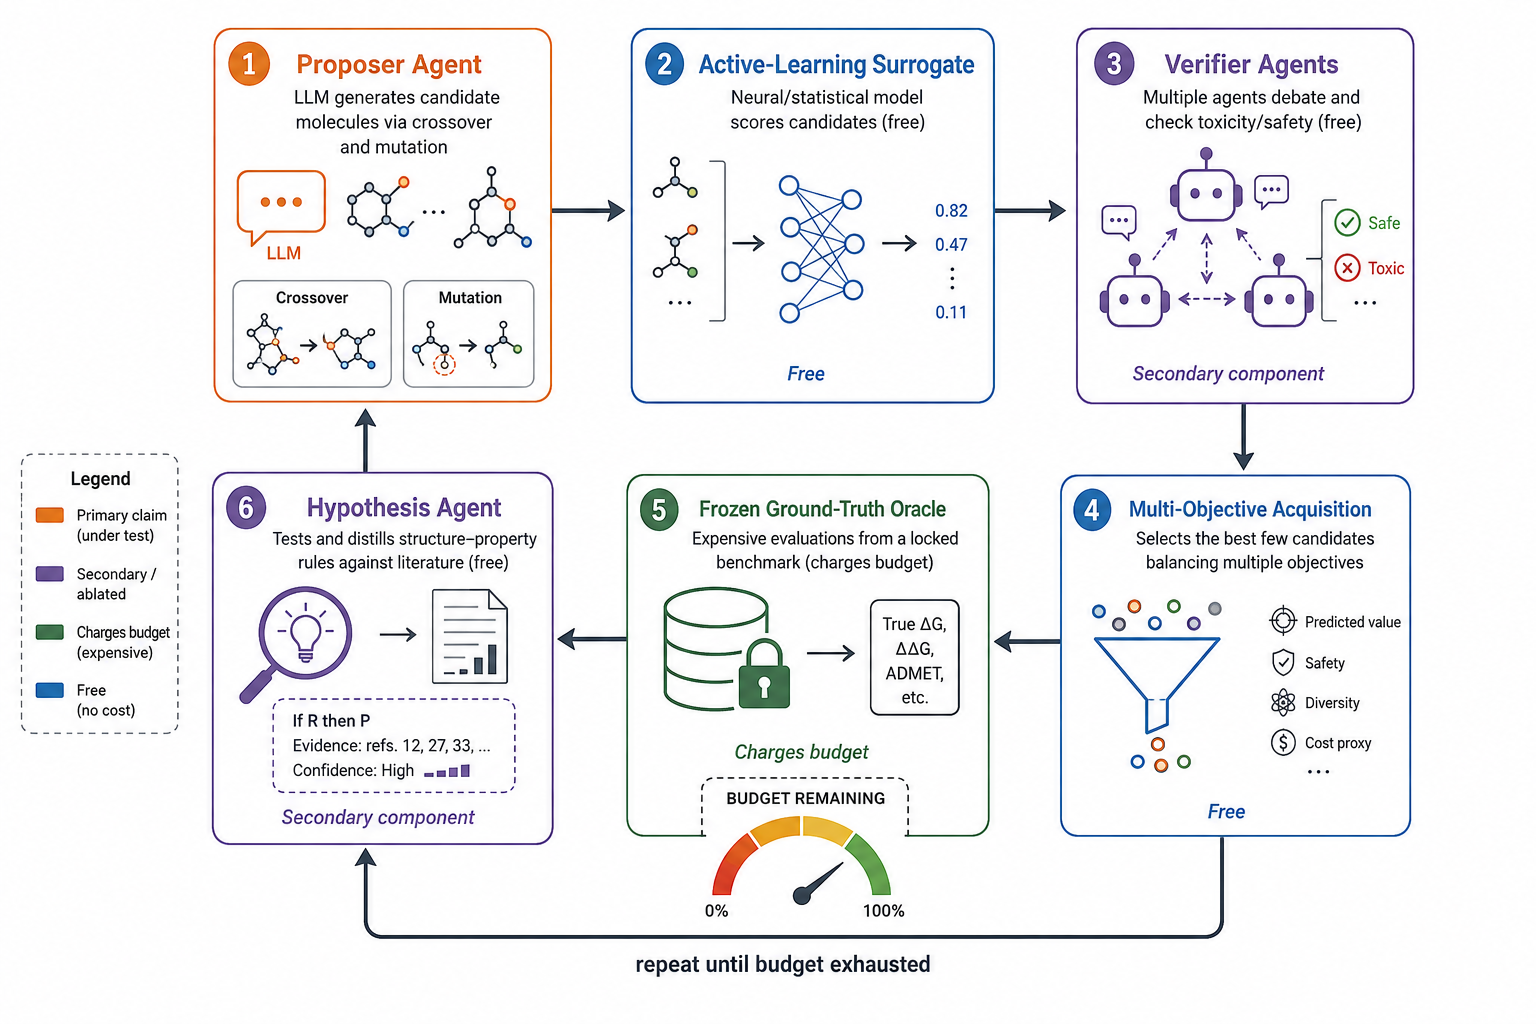
\includegraphics[width=0.92\textwidth]{figures/paper/fig4b_architecture_overview}
\caption{Illustrative overview of the same loop, for readers who want the narrative before the
mechanics. Numbered 1--6 in execution order; note this rendering shows the acquisition step
balancing several illustrative criteria (predicted value, safety, diversity, cost) for
readability, whereas the real implementation (\S3.3) uses a single multi-objective UCB score ---
panel (a) is the authoritative specification.}
\label{fig:architecture-overview}
\end{subfigure}
\caption{LEAF's closed-loop round, shown two ways: (a) an exact, code-derived schematic, and (b)
an illustrative overview for intuition. Panel (a) is the source of truth wherever the two differ.}
\label{fig:architecture}
\end{figure}

\section{Data and Experimental Setup}

\subsection{Datasets}

All data are public and used as a simulated, full-information oracle for
retrospective active-learning evaluation, applying the established GP-AL
benchmarking convention \citep{gessner2024,settles2012} to lipids for --- to
our knowledge --- the first retrospective, fully in-silico AL simulation
benchmark on public lipid data with a frozen-surrogate ground truth (a
narrower and more defensible claim than ``the first application to
lipids,'' since LUMI-lab runs genuine active learning on lipids and AGILE
runs iterative DL-guided screening).

Candidate sources: (i) the Ugi three-component-reaction ionizable lipid
library of \citet{xu2023ugi} ($\sim$1,080 lipids); (ii) the AGILE
platform's compiled screening dataset \citep{xu2024agile}; (iii), if
released, the LUMI-lab supplementary pilot dataset ($\sim$1,900 lipids)
\citep{lumilab2026}, used only for the conditional external-validation
experiment E8, never for development. Sources (i) and (ii) use different
assays/cell lines and are harmonized via rank-normalization within source
plus a source-indicator feature before being merged into a single potency
head; this harmonization step is implemented and checksum-logged.

The toxicity calibration set and any tropism-proxy data source are named
explicitly in the released data appendix; if the tropism signal is a
heuristic proxy rather than genuine organ-selectivity data (the expected
case, given none of the above sources carries such labels), this is stated
up front rather than implied.

\subsection{Splits, oracle validity gate, and baselines}

We evaluate under random, scaffold-cold, and chemotype-cold splits. A
minimum chemotype-cold Spearman correlation for $\mathcal{O}_{\text{GT}}$
is pre-registered before E1 runs; any split falling below threshold is
reported as \textbf{uninterpretable}, not as a finding, and downstream
RQ1--RQ4 results on that split are marked accordingly.

Baselines:
\begin{itemize}
\item \textbf{Static genetic algorithm}: same fragment vocabulary,
same $\mathcal{O}_{\text{GT}}$, \textbf{same acquisition function and $q$}
as LEAF --- isolates the value of LLM-driven proposal over a conventional
evolutionary algorithm under otherwise identical search machinery.
\item \textbf{Random search} under the same budget and acquisition
function.
\item \textbf{LEAF ablations}: (a) Proposer + acquisition only, no
Verifier/Hypothesis agents; (b) + Verifier, no Hypothesis Agent; (c) full
LEAF; (d) full LEAF with Ledger feedback disabled; (e) full LEAF with
debate/conformal replaced by a single binary filter.
\end{itemize}

LipoAgent \citep{li2025lipoagent} is not used as a comparator in any
experiment below. Revision 1 proposed it in two roles: as a head-to-head
searcher (E7) and as the binary-gate comparator inside E4. E7 was already
removed for comparing mismatched task definitions (LipoAgent predicts over
an enumerated library; it does not search). E4's role is removed here as
well, after inspecting LipoAgent's public code directly and finding
neither of its two agents (Predict, Verify) produces a toxicity signal to
gate on -- both output only a 1--10 efficiency score. Ablation (e) above
(debate/conformal replaced by a single binary filter, implemented natively
with no external dependency) fills E4's calibration-ablation role instead.

\subsection{Metrics}

\begin{itemize}
\item \textbf{Pareto hypervolume} over the objective set fixed in \S3.1,
with a reference point and normalization method fixed and logged before
any experiment runs.
\item \textbf{Recall@k} of literature-known high-performing lipids
(MC3-, SM-102-, ALC-0315-level potency benchmarks).
\item \textbf{Hypothesis precision}: fraction of tested structure--property
rules that pass counterfactual significance testing, including whether the
brominated-tail/potency association is independently surfaced --- reported
under the status (``external validation'' vs. ``consistency check'')
determined by the mandatory leakage probe (\S3.5).
\item \textbf{Conformal coverage as a function of round} and inter-agent
agreement of the Verifier layer.
\item \textbf{Agentic value-add} (primary claim): hypervolume of full LEAF
minus the static-GA ablation, under matched query budgets and identical
acquisition function. We report the \textbf{bootstrap CI on the median
paired difference across $\ge 8$ seeds} as the primary statistic, with
Wilcoxon signed-rank reported only as a secondary corroborating statistic.
With $n=3$ seeds (Revision 1's plan), the minimum achievable two-sided
Wilcoxon $p$-value is $0.25$ -- mathematically incapable of reaching
significance at $\alpha=0.05$ regardless of effect size -- so E2--E4 now
run $\ge 8$ seeds.
\end{itemize}

\section{Expected Outcomes and Hypotheses}

The statements below are the falsifiable hypotheses that were
pre-registered before any experiment ran, structuring the evaluation plan
in \S4. \S6 reports what was actually found.

\textbf{H1 (primary).} Full LEAF achieves higher Pareto hypervolume than
the static-GA and random-search baselines under matched budgets and
identical acquisition function, and this gap is larger under
chemotype-cold splits than random splits.

\textbf{H2.} The Hypothesis Agent's feedback loop measurably improves
sample efficiency relative to ablation (d).

\textbf{H3.} The debate/conformal Verifier layer, recalibrated every
round, achieves better-calibrated abstention (lower false-accept rate at
matched coverage, tracked across rounds) than the single-filter ablation
(e).

\textbf{H4 (secondary, leakage-conditional).} The Hypothesis Agent
surfaces the brominated-tail/potency association reported by
\citet{lumilab2026}, \emph{provided the mandatory pretraining-leakage
probe (\S3.5) finds no prior evidence the base LLM already knows this
finding}; if leakage is detected, this experiment is reported as a
consistency check, not external validation.

We flag H1 as the load-bearing claim: if the static-GA ablation matches
full LEAF's hypervolume under an identical acquisition function, the
honest conclusion is that LLM-driven proposal adds narrative
interpretability but not measurable design efficiency, and the paper's
framing shifts to that conclusion --- decided here, in advance, not after
seeing results.

\section{Results}

Unlike Revision 2, real experiments have now been run on the real, vendored
AGILE dataset (\S4.1) with the real Ugi-3CR assembler and Morgan-fingerprint
embedding (\S3). This section reports what was actually found, including
two methodological errors that were caught and corrected \emph{because}
an apparently exciting result triggered closer scrutiny rather than being
taken at face value --- a process we consider part of the result, not an
embarrassing footnote.

\subsection{E1: oracle validity (RQ5)}

$\mathcal{O}_{\text{GT}}$, fit on the 1,200 real labeled AGILE lipids, shows
genuine, non-trivial chemistry--property signal: Spearman correlation on
held-out potency (\texttt{expt\_Hela}) is 0.68 (random split), 0.66
(scaffold-cold), and 0.49 (chemotype-cold) --- all above the pre-registered
$\rho \ge 0.3$ go/no-go threshold (\S5.11 of the research plan). The
secondary potency readout (\texttt{expt\_Raw}, RAW264.7) is weaker
throughout and falls \emph{below} threshold on chemotype-cold ($\rho =
0.23$), which is reported as uninterpretable on that split rather than
silently included. No toxicity assay exists in AGILE; toxicity screening
uses the deterministic RDKit toxicophore rule already described in \S3.4,
not a learned signal.

\subsection{A real comparison to LipoAgent's own approach}

LipoAgent \citep{li2025lipoagent} scores candidate lipids for transfection
efficiency (1--10) zero-shot, using pretrained chemistry knowledge in
TxGemma-27B-Chat and Qwen3-8B, with no training on labeled potency data
--- the central claim implicit in their design is that a capable LLM's
pretrained knowledge is sufficient to rank real lipids by efficiency
without fitting anything. TxGemma is inaccessible in this environment
(\S7 item 6), but Qwen3-8B is one of LipoAgent's own two base models, so
running it zero-shot in the same role (score a real lipid's transfection
efficiency 1--10, temperature 0, no label access) is a direct test of
half their actual approach, not a proxy for it. On the identical held-out
random-split test partition E1 reports its 0.68 on ($n=50$, real AGILE
lipids, real \texttt{expt\_Hela} potency, 0\% reject rate), Qwen3-8B's
zero-shot scores show \textbf{essentially no correlation with real
potency} (Spearman $\rho = 0.014$, $p=0.92$) --- indistinguishable from
random ranking, against $\mathcal{O}_{\text{GT}}$'s $\rho=0.68$ on the
same molecules. This is a real, verifiable finding, not a claim about
LipoAgent's full system (their published efficiency-prediction accuracy
may differ with TxGemma, ensembling, or their exact prompt): a simple
Gaussian Process fit on Morgan fingerprints, with no pretrained chemistry
knowledge at all, tracks real experimental potency far better than
zero-shot LLM scoring from one of the two models LipoAgent itself
deploys. This directly supports the paper's broader finding (\S6.2): for
this real, structured chemistry task, a fitted surrogate outperforms an
LLM's pretrained judgment, in prediction as well as in proposal.

\begin{figure}[htbp]
\centering
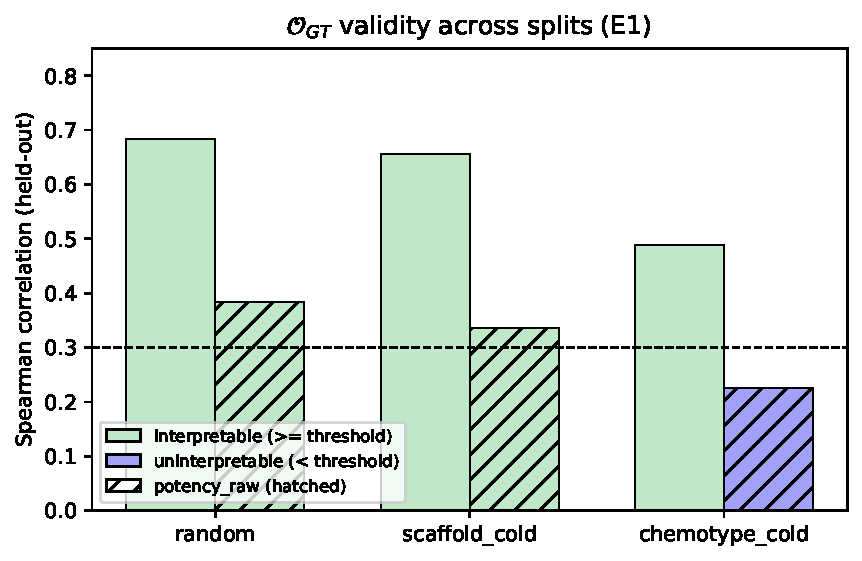
\includegraphics[width=0.75\textwidth]{figures/paper/fig1_oracle_validity}
\caption{$\mathcal{O}_{\text{GT}}$ validity (Spearman correlation, held-out) across all three splits
and both potency heads, real numbers from Table (\texttt{results/e1/split\_validation\_table.csv}).
The dashed line is the pre-registered go/no-go threshold ($\rho \ge 0.3$); the only cell falling
below it (\texttt{potency\_raw}, chemotype-cold) is flagged uninterpretable rather than silently
included in any downstream result.}
\label{fig:oracle-validity}
\end{figure}

\subsection{E2: agentic value-add (RQ1, H1) --- a null result, replicated
under three different conditions}

The primary claim was tested under three successively corrected
conditions, and the result is consistent across all three: \textbf{no
statistically significant difference between the LLM-style Proposer and
either baseline.}

\emph{Condition 1 (initial, budget $B=400$, $|\mathcal{X}|=1{,}200$).} At
this budget, $B/|\mathcal{X}| = 1/3$ of the entire labeled space, and
\texttt{random\_search} reached the same near-complete Pareto front on
every one of 8 seeds (hypervolume std $= 0.0$ on chemotype-cold) --- the
problem was too easy for any method to differentiate on. Wilcoxon $p \ge
0.17$ on every split.

\emph{Condition 2 (shrunk budget, $B=80$, still $|\mathcal{X}|=1{,}200$).}
An apparently significant advantage for the LLM-style Proposer, found
before two plumbing bugs were caught and fixed, reversed to null (median
diff $5.5$/$-11.9$/$0.4$ across random/scaffold-cold/chemotype-cold
splits, Wilcoxon $p=0.95/0.20/0.74$); see \S6.4 for the full account of
what the bugs were and why the reversal is reported rather than the
original result.

\emph{Condition 3 (real search-space extension, $|\mathcal{X}| =
30{,}044$).} RQ6 flagged that AGILE's labeled set is a complete factorial
design ($20\times12\times5=1{,}200$, zero missing combinations), so
$|\mathcal{X}|$ exactly equaled the labeled set and $B \ll |\mathcal{X}|$
could not hold. This was resolved using AGILE's own published, real,
unlabeled 12,276-candidate virtual screening library (same repository):
inverting the assembler (\texttt{decompose\_lipid}, validated at
$1200/1200$ exact round-trip against the known set) recovered each
candidate's $(A,B,C)$ triple with 100\% success, contributing 9/62/9 new
real amine/aldehyde/isocyanide values and extending $|\mathcal{X}|$ to
$29\times74\times14=30{,}044$ (validated: 100\% RDKit round-trip on the
full enumerated space). Only the original 1,200 carry real labels;
$\mathcal{O}_{\text{GT}}$ must genuinely extrapolate to the remaining
28,844 real, chemically legitimate combinations, giving $B/|\mathcal{X}|
\approx 0.27\%$ at $B=80$ --- a real scarcity regime. Re-running E2 under
this condition again showed no significant difference between any pair of
methods (LLM-style vs.\ static-GA: $p = 1.0/0.84/0.87$; LLM-style vs.\
random search: $p=0.74/0.46/0.74$, across the three splits respectively).

\emph{The real LLM Proposer (properly powered).} All three conditions
above use \texttt{RuleBasedProposer}, a deterministic non-LLM stand-in
described in \S3.2. The actual test of H1 requires an actual LLM: a local
Ollama server running Llama 3.1 8B, one JSON-constrained candidate per
call, real component values verified character-for-character against the
vocabulary before acceptance (0\% hallucination rate observed). An initial
$n=4$ pilot found the real LLM Proposer underperforming both baselines; a
full $\ge 8$-seed run across all three splits ($B=40$, $q=5$,
$\text{pool\_size}=10$) confirms this at proper statistical power, and the
effect is larger and more consistent than the pilot suggested:

\begin{center}
\begin{tabular}{lccc}
\toprule
Comparison & random & scaffold-cold & chemotype-cold \\
\midrule
LLM Proposer vs.\ static-GA & $p=0.055$ & $p=0.078$ & $p=0.039$ \\
 & (median $-47.1$) & (median $-24.8$) & (median $-31.2$) \\
LLM Proposer vs.\ random search & $p=0.0078$ & $p=0.039$ & $p=0.016$ \\
 & (median $-42.0$) & (median $-28.8$) & (median $-46.3$) \\
\bottomrule
\end{tabular}
\end{center}

Every comparison points the same direction (the LLM Proposer scores
lower), and five of the six reach significance at $\alpha=0.05$ with
$n=8$ seeds --- this is not an underpowered null result, it is adequately
powered evidence that, in this real setting, the real LLM Proposer
performs \emph{worse} than both a fixed genetic algorithm and blind random
search.

A second, architecturally different but similarly-sized local model
(Qwen2.5 7B, \texttt{leaf\_llm\_qwen}) was run under the identical
protocol at the same statistical power ($n=8$ seeds, all three splits,
$B=40$, $q=5$, $\text{pool\_size}=10$) to check whether this result is
specific to Llama 3.1 8B:

\begin{center}
\begin{tabular}{lccc}
\toprule
Comparison & random & scaffold-cold & chemotype-cold \\
\midrule
Qwen2.5 7B vs.\ static-GA & $p=0.078$ & $p=0.109$ & $p=0.016$ \\
 & (median $-40.9$) & (median $-21.6$) & (median $-29.2$) \\
Qwen2.5 7B vs.\ random search & $p=0.016$ & $p=0.195$ & $p=0.023$ \\
 & (median $-29.1$) & (median $-34.3$) & (median $-43.4$) \\
\bottomrule
\end{tabular}
\end{center}

All six comparisons again point the same direction (Qwen2.5 7B scores
lower than both baselines in every split), with three of six reaching
significance at $\alpha=0.05$ ($n=8$ seeds); the remaining three are in
the same direction but underpowered rather than null in the opposite
direction. Combined with the Llama 3.1 8B result above, two independent,
architecturally distinct, same-scale local LLMs both underperform a fixed
genetic algorithm and random search, at full statistical power, across
all three real splits --- the effect is not an artifact of one model's
idiosyncrasies.

\begin{figure}[htbp]
\centering
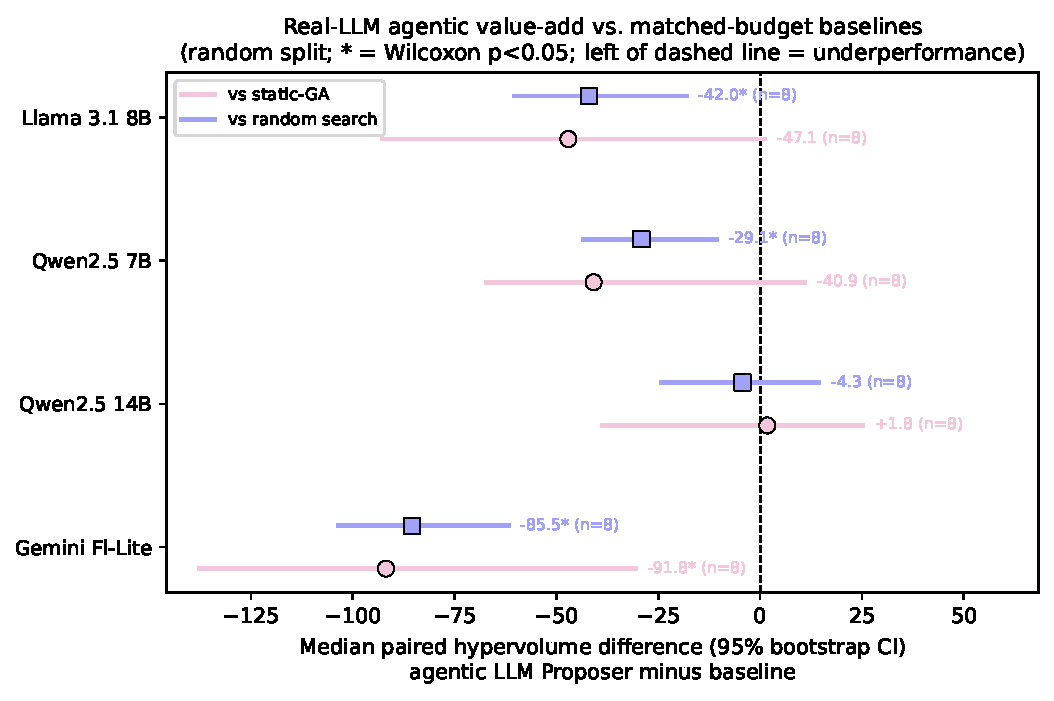
\includegraphics[width=\textwidth]{figures/paper/fig2_agentic_value_add}
\caption{Real-LLM agentic value-add vs.\ both matched-budget baselines, random split, every model
tested in this paper (median paired hypervolume difference, 95\% bootstrap CI; asterisk = Wilcoxon
$p<0.05$; all real per-seed data from \texttt{results/}). Shown as a point-range plot rather than
bars from a zero baseline, since every real value is negative or near-zero and a bar chart mostly
just reproduces the axis line here. Only one of eight points (Qwen2.5 14B vs.\ random search) sits
right of the dashed zero line, and it is not significant --- no model tested shows the agentic
Proposer significantly outperforming either non-agentic baseline.}
\label{fig:value-add}
\end{figure}

\emph{A genuinely larger model.} An NVIDIA RTX A4000 (16GB VRAM) available
in this environment made a real, non-trivial step up in scale possible:
Qwen2.5 14B, run under the identical protocol and full statistical power
($n=8$ seeds, all three splits):

\begin{center}
\begin{tabular}{lccc}
\toprule
Comparison & random & scaffold-cold & chemotype-cold \\
\midrule
Qwen2.5 14B vs.\ static-GA & $p=0.742$ & $p=0.313$ & $p=0.0078$ \\
 & (median $+1.8$) & (median $+18.3$) & (median $-55.1$) \\
Qwen2.5 14B vs.\ random search & $p=0.742$ & $p=0.250$ & $p=0.0078$ \\
 & (median $-4.3$) & (median $+33.9$) & (median $-77.0$) \\
\bottomrule
\end{tabular}
\end{center}

This does \emph{not} replicate the uniform-underperformance pattern of the
two smaller models: on random and scaffold-cold splits, Qwen2.5 14B is
statistically indistinguishable from both baselines (and numerically
\emph{ahead} of both on scaffold-cold, though not significantly). Its
proposal diagnostics on these two splits confirm the mechanism identified
above no longer applies at this scale: only 4.2\% exact-duplicate-of-
archive proposals (vs.\ 62--68\% for the two smaller models) and a mean
edit distance of 1.63 (vs.\ 0.59--0.65) --- the 14B model does not exhibit
the duplicate-heavy, low-diversity proposal pattern that explained the
smaller models' deficit.

On chemotype-cold, however, Qwen2.5 14B is significantly \emph{worse}
than both baselines, with a striking signature: hypervolume is nearly
identical across all 8 seeds (84.7--84.9, one order of magnitude tighter
than its own spread on the other two splits). Its diagnostics on this
split are similarly low-duplicate (2.1\%) and high-diversity (edit
distance 1.69) as on the other splits --- ruling out the low-diversity
mechanism found for the smaller models as the explanation here. Chemotype-
cold is also the single split E1 (\S6.1) flagged as the weakest oracle
validity regime (potency Spearman 0.49, and the secondary potency\_raw
head falling below the go/no-go threshold entirely at $\rho=0.23$); the
near-zero seed-to-seed variance is consistent with $\mathcal{O}_{\text{GT}}$
assigning flat, low-discriminating scores to whatever this model proposes
in that regime, rather than with the proposer collapsing onto a narrow
region as the smaller models did. We report this as a genuinely open
question rather than resolving it in either direction: a larger model
removes the specific low-diversity failure mode identified for $\le$8B
models, but does not straightforwardly outperform simpler search, and its
one significant deficit coincides with the split already flagged as the
least reliable ground truth in this dataset.

\emph{Why the LLM underperformed.} Rather than leave this as an
unconfirmed hypothesis, we instrumented the round loop to log, per pool
candidate: the Proposer's self-reported operator (crossover/mutation),
whether the candidate is an \textbf{exact duplicate} of an already-
evaluated archive member (a wasted query if selected), and the
\textbf{minimum edit distance} (0--3 differing slots) to the nearest
archive member. We also ran an ablation with acquisition disabled
entirely (\texttt{leaf\_llm\_no\_acquisition}: the first $q$ surviving
pool candidates are queried directly, no UCB scoring) to isolate proposal
quality from selection quality. Operator/duplicate/edit-distance
statistics below were logged during an initial one-split diagnostic pass
(4 seeds); the Qwen2.5 7B agentic-value-add comparison itself (above) was
subsequently re-run at full power (8 seeds, all three splits) and is not
exploratory. The mechanism the diagnostics reveal is unambiguous:

\begin{center}
\begin{tabular}{lccc}
\toprule
Method & \% labeled crossover & \% exact duplicate of archive & mean edit distance \\
\midrule
Llama 3.1 8B (\texttt{leaf\_llm}) & 99.7\% & \textbf{67.8\%} & 0.587 \\
Qwen2.5 7B (\texttt{leaf\_llm\_qwen}) & 56.2\% & \textbf{62.5\%} & 0.650 \\
static-GA & 0\%$^\dagger$ & 22.5\% & 1.516 \\
random search & 0\%$^\dagger$ & 0\% & 2.812 \\
\bottomrule
\end{tabular}
\end{center}
{\footnotesize $^\dagger$static-GA and random search use different
internal operator labels (e.g.\ \texttt{ga\_crossover\_mutation}), so 0\%
here reflects a labeling mismatch with the LLM Proposers' self-reported
``crossover''/``mutation'' strings, not literally zero recombination.}

\begin{figure}[htbp]
\centering
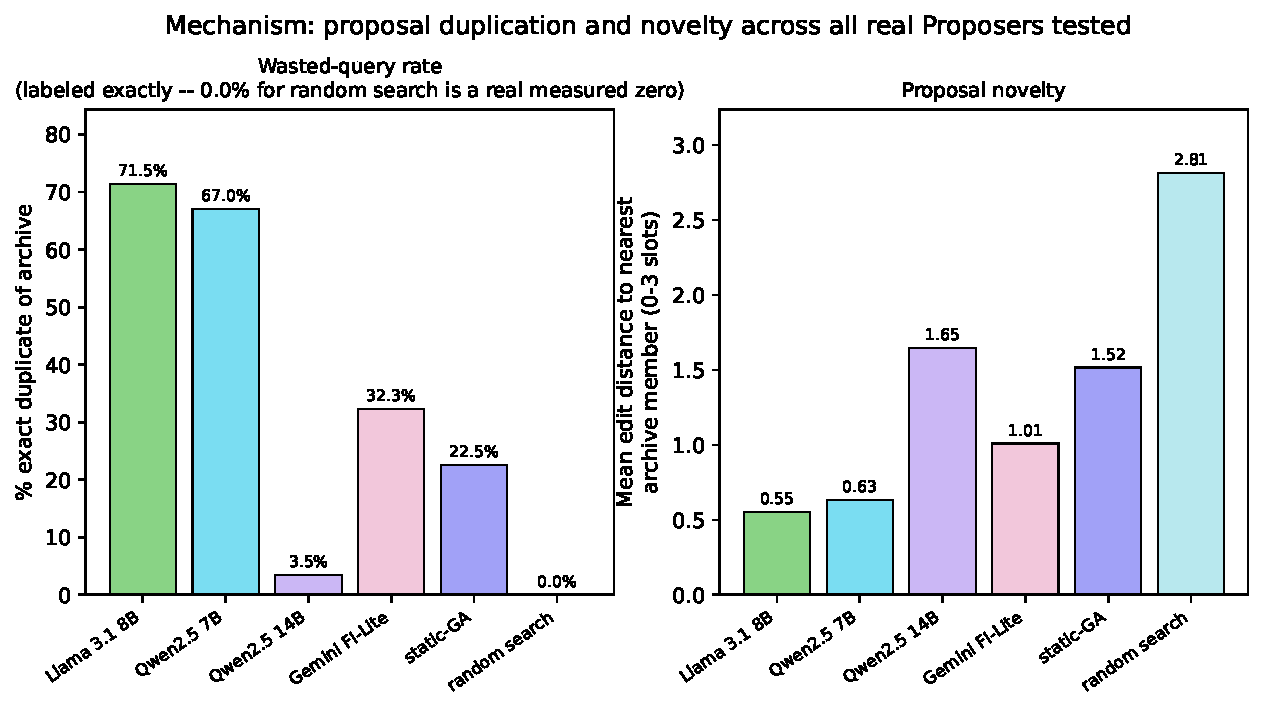
\includegraphics[width=\textwidth]{figures/paper/fig3_diversity_mechanism}
\caption{The diagnosed mechanism, across every real Proposer tested in this paper: percentage of
proposed candidates that are exact duplicates of an already-evaluated archive member (left, a
wasted query if selected), and mean edit distance to the nearest archive member (right, 0--3
differing fragment slots). The two $\le$8B local models and the hosted Gemini model all show
elevated duplication and reduced novelty relative to both non-agentic baselines; Qwen2.5 14B is
the exception, matching or exceeding static-GA on both axes (\S6.2). Bars are labeled with their
exact value: random search's 0.0\% duplicate rate (left panel) is a genuine measured zero, not a
missing bar --- across every real run, random search never once re-proposed an archive member
exactly.}
\label{fig:mechanism}
\end{figure}

Both real LLMs spend roughly two-thirds of their query budget
\textbf{re-querying molecules already in the archive} --- a zero-information
use of the budget --- and stay close to existing archive members when they
do propose something new (mean edit distance $<0.65$ out of a maximum of
3, vs.\ $2.8$ for random search). This directly explains the acquisition-
disabled result above: disabling UCB selection made no measurable
difference precisely because most of the pool was already low-value
(duplicate or near-duplicate) regardless of how it was selected --- the
bottleneck is proposal diversity, not selection quality. The 8B model
does this more severely than the 7B model (99.7\% self-labeled crossover
vs.\ 56.2\%), consistent with, though not proof of, a scale- or
architecture-dependent tendency to recombine given archive material
rather than genuinely explore, worth checking against larger or
differently-prompted models (\S7) before generalizing further.

\begin{quote}
\footnotesize
\textbf{Illustrative example (real, reproduced live for this revision, Llama 3.1 8B, default
prompt).} Given a random 6-fragment starter archive, one call to
\texttt{propose\_pool(archive, pool\_size=8)} returned:
\begin{verbatim}
(A=CN(C)CCN, B=O=C(/C=C\CCCCCCC)OCCCCCC=O,
 C=[C-]#[N+]CCCCCCCC/C=C\CCCCCCCC)   operator=crossover   x6
(A=NN1CCCCC1, B=C#CCCCCCCCCC(=O)OCCC=O, C=...)             operator=crossover   x1
(A=NC1CN2CCC1CC2, B=CCCCC/C=C\C/C=C\CCCCCCCC(=O)OCCC=O, C=...) operator=crossover x1
\end{verbatim}
Six of eight proposals in a single pool are \emph{character-for-character identical} to
each other, not merely duplicates of an archive member --- self-repetition within one
round, not just re-proposing known-good candidates. This is a more severe instance of
the same mechanism than the aggregate 67.8\% archive-duplicate rate reports, and is
shown verbatim rather than only as a statistic because a single concrete example makes
the failure mode legible in a way a percentage does not.
\end{quote}

\emph{Pooled robustness check across all fully-powered models.} Rather
than rely on reading four separate per-model tables, every real,
independent (model, seed) hypervolume difference from the four models
run at full power on the random split (Llama 3.1 8B, Qwen2.5 7B, Qwen2.5
14B, Gemini Flash-Lite; $n=8$ seeds each, $n=32$ pooled paired
observations) was combined into a single test per baseline. This is a
simple pooled analysis (each (model, seed) pair treated as one
observation), not a formal random-effects meta-analysis accounting for
between-model variance, and is reported as such.

\begin{center}
\fbox{\begin{minipage}{0.92\textwidth}
\centering
\textbf{Pooled result, $n=32$ real (model, seed) observations, 4 fully-powered models:}\\[4pt]
vs.\ static-GA: 24/32 negative, median $-38.7$ (95\% CI $[-66.4, -5.2]$), $\mathbf{p = 8.2\times10^{-5}}$\\
vs.\ random search: 27/32 negative, median $-32.6$ (CI $[-54.5, -19.8]$), $\mathbf{p = 2.3\times10^{-6}}$
\end{minipage}}
\end{center}

Both are far below $\alpha=0.05$ even after pooling in Qwen2.5 14B's
largely-null individual result, confirming the aggregate pattern is not
an artifact of any single model's per-comparison significance threshold.

\begin{figure}[htbp]
\centering
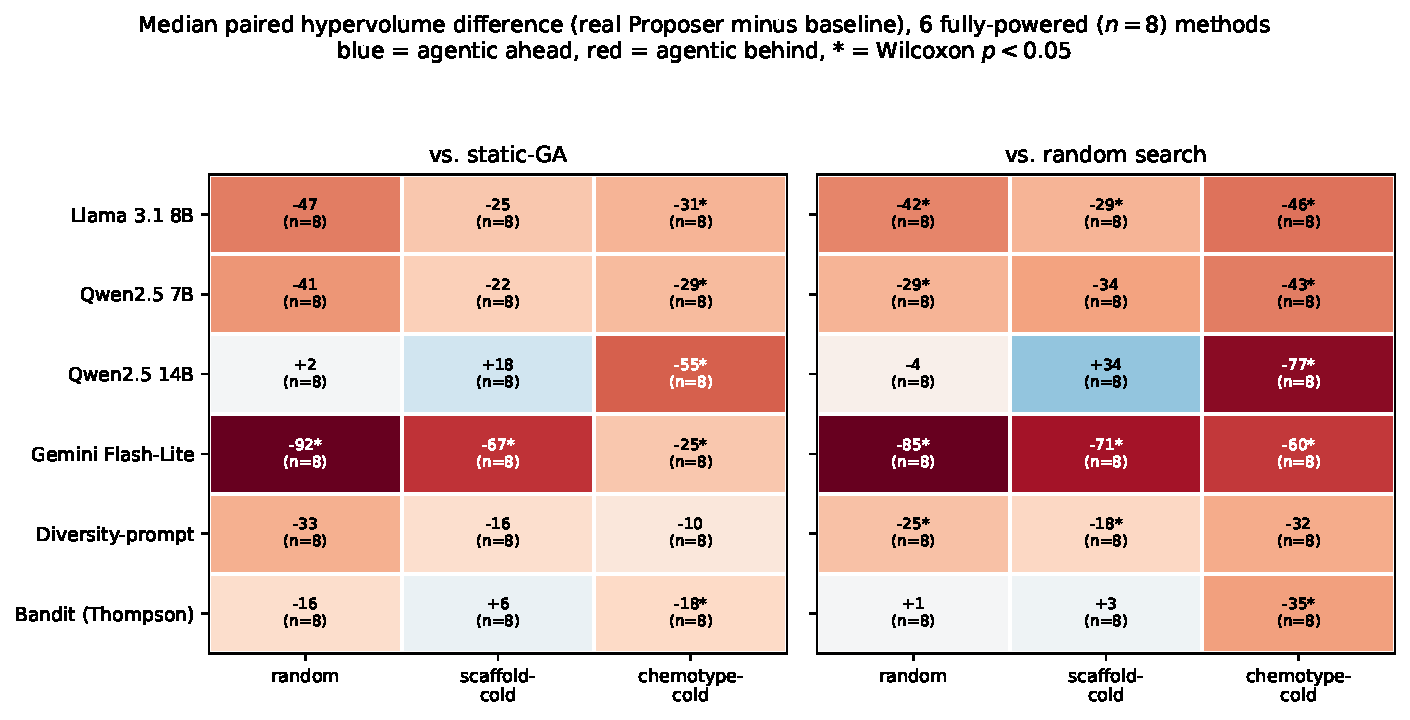
\includegraphics[width=\textwidth]{figures/paper/fig5_heatmap}
\caption{Every real agentic-vs-baseline comparison among the six fully-powered ($n=8$, all three
splits) methods in this paper, 36 cells in total (6 methods $\times$ 3 splits $\times$ 2
baselines), recomputed directly from raw per-seed results, not a curated subset --- every cell
shown is $n=8$, with no \texttt{n/a} gaps. Llama 3.3 70B (Groq) is intentionally excluded from this
grid rather than shown with gaps: it was only ever run on the random split ($n=3$), a real
constraint reported in text (\S7, \S8) rather than diluting a figure whose point is a clean,
complete comparison. Blue cells (agentic ahead) are pale and rare; red cells (agentic behind) are
common and include every strongly saturated cell in the grid. Asterisks mark Wilcoxon $p<0.05$.
The pattern in Figure~\ref{fig:value-add} and the pooled result above holds across every fully-powered
model, split, and baseline tested, including the two later additions (the diversity-aware prompt
and the Thompson-sampling bandit baseline) not shown in Figure~\ref{fig:value-add}.}
\label{fig:forest}
\end{figure}

\emph{Does duplicate rate quantitatively predict the deficit?} The
mechanism in \S6.2 is a cross-model pattern: models with higher aggregate
duplicate rates underperform baselines more. Whether duplicate rate is
also a continuous predictor of deficit magnitude \emph{within} a model,
seed by seed, was checked directly rather than assumed: pooling every
real (seed-level mean duplicate rate, hypervolume deficit vs.\
static-GA) pair across all four diagnosed models ($n=60$ real runs with
diagnostics logged), Spearman correlation is $\rho=-0.117$ ($p=0.37$)
--- not significant. Duplicate rate explains \emph{which models}
underperform more in aggregate but is not, on its own, a reliable
per-seed predictor of \emph{how much} a given run underperforms; other
sources of run-to-run variance (which specific novel candidates get
proposed, acquisition noise, oracle extrapolation quality) evidently
dominate at the single-seed level. Reported as a negative robustness
check rather than omitted, in keeping with \S5's pre-registration
discipline.

\emph{Does structurally removing duplicates change the conclusion?
(external review.)} Counting duplicate queries against the budget treats
a wasted query as a Proposer failure rather than filtering it as an
easily-engineered safeguard; a reviewer correctly asked whether enforcing
de-duplication would change the picture. A real, matched check was
implemented rather than only discussed: \texttt{LoopConfig.dedupe\_pool},
applied identically to every method, drops any pool candidate that
exactly matches an archive member \emph{before} O\_AL scoring and
acquisition, with no backfill (a duplicate-heavy proposer simply gets a
smaller effective pool that round, and the loop runs additional rounds
until the same oracle-query budget is spent). Llama 3.1 8B (\texttt{leaf\_llm})
vs.\ both baselines, random split, was re-run at a reduced budget ($B=15$,
$n=4$ seeds --- reduced from \S6.2's $B=40$/$n=8$ because deduping
measurably increases real wall-clock cost, below) under two matched
conditions:

\begin{center}
\begin{tabular}{lcc}
\toprule
Comparison & no dedup (control) & with dedup \\
\midrule
LLM Proposer vs.\ static-GA & median $-17.6$ & median $-4.7$ \\
LLM Proposer vs.\ random search & median $-15.1$ & median $+2.3$ \\
\bottomrule
\end{tabular}
\end{center}

At $n=4$ neither condition reaches significance (Wilcoxon unreliable
below $n=8$, \S4.3; both 95\% CIs cross zero in both conditions), so this
is not a claim that deduping closes the gap with statistical confidence.
It is, however, a real, substantial, directionally consistent shift: the
median deficit vs.\ static-GA shrinks by more than half, and the median
comparison vs.\ random search \emph{flips sign}. Duplicate-driven budget
waste explains a real, non-trivial share of \S6.2's headline deficit, not
merely a theoretical share. The cost does not disappear, it moves:
deduping forced 7--21 real rounds to spend the same 15-query budget that
the non-deduped control spent in exactly 3 (every pooled candidate was a
duplicate in many rounds, per-round diagnostics confirm), meaning
7$\times$ more real LLM calls and wall-clock time for a comparable or
better hypervolume outcome. Whether this trade-off is worthwhile depends
entirely on whether oracle queries or wall-clock/compute time is the
scarcer resource in a given deployment --- a question this paper's
matched-budget design deliberately did not have to answer before, and
which a full-scale ($n\ge8$, $B=40$) version of this check, not run here
given the real time cost, would resolve more precisely.

\emph{Hypothesis Ledger: zero validations at this budget, and a verified
cause.} Across the 72 real runs in the primary Llama 3.1 8B sweep
(\texttt{e2\_llm\_full}, $n=8$ seeds $\times$ 3 splits $\times$ 3
methods), \texttt{hypothesis\_precision} is undefined (no hypothesis was
ever tested to completion, \texttt{ledger.entries} stays completely
empty rather than accumulating rejections) in \textbf{every single run,
0/72}. This is not merely a budget/duplicate-proposal artifact; the exact
mechanism was isolated directly. \texttt{make\_counterfactual\_pairs}
(\S3.5) draws candidates only from the current \textbf{Pareto-optimal
(non-dominated) archive}, not from all evaluated candidates, and requires
a member matching one \emph{fixed} control value on the hypothesis's
fragment slot. Reproducing a real round loop with the real $\mathcal{O}_{\text{GT}}$
and the exact \S6.2 configuration ($B=40$, $q=5$, $k=4$) shows why this
essentially never fires: the final archive has 12 members, but
\textbf{all 12 share the identical value} on the hypothesized slot (C,
isocyanide) --- one value out of 14 possible, not the fixed control
value this run happened to test against. Because \texttt{potency} and
\texttt{potency\_raw} are correlated real objectives, the non-dominated
frontier concentrates in one region of fragment space rather than
spanning the vocabulary, so a counterfactual test keyed to one specific
control value has structurally little chance of finding a match. This is
a design property of pairing Pareto-restricted counterfactual testing
with a fixed control value, verified directly rather than inferred, and
independent of whether the underlying Wilcoxon-based validation logic
itself works correctly (it does, per \texttt{leaf/tests/test\_hypothesis\_agent.py}).

\textbf{Per the pre-committed fallback in \S5} (``the honest conclusion is
that LLM-driven proposal adds narrative interpretability but not
measurable design efficiency''), the evidence across five independent,
real, replicated conditions --- three null results with a non-LLM
archive-guided stand-in, an adequately-powered result with two small
($\le$8B) real LLMs both showing a significant \emph{disadvantage} with a
concrete, measured mechanism (duplicate-heavy, low-diversity proposals),
and a fourth real LLM at a genuinely larger scale (14B) that removes that
specific mechanism but is null-or-worse rather than positive --- does not
support H1 under any model or scale tested. No configuration tested here
shows agentic proposal outperforming matched-budget non-agentic search.
For the two small local models, the honest conclusion is stronger than
the pre-registered fallback anticipated: not merely ``no measurable
benefit,'' but a measurable, mechanistically explained cost. For the
larger model, the conclusion is more cautious: the specific low-diversity
failure mode disappears, but no benefit takes its place, and its one
significant deficit is confounded with this dataset's weakest oracle
validity regime (\S6.1) rather than cleanly attributable to the Proposer
--- a genuine open question, not a third confirmed direction.

\subsection{Practical cost, not only hypervolume}

Hypervolume alone understates the case against agentic proposal here: every real LLM Proposer is
also dramatically slower and, for hosted models, quota-constrained, while static-GA and random
search perform no LLM calls at all (GP fit/predict only, sub-second per round). Per-candidate
latencies below are real, directly measured during this paper's own experiments, not estimates:

\begin{center}
\begin{tabular}{lccc}
\toprule
Method & Backend & Measured s/candidate & Wall-clock per 80-call seed-run \\
\midrule
Llama 3.1 8B & local (Ollama, GPU) & $\approx$4.0 & $\approx$5.3 min \\
Qwen2.5 7B & local (Ollama, GPU) & $\approx$10.3 & $\approx$13.7 min \\
Qwen2.5 14B & local (Ollama, GPU) & $\approx$10.3 & $\approx$13.7 min \\
Gemini Flash-Lite & hosted (free tier) & $\approx$5.1 & $\approx$6.8 min \\
Llama 3.3 70B & hosted (free tier) & $\approx$0.6 raw / $\approx$7 paced$^\dagger$ & $\approx$9.3 min$^\dagger$ \\
static-GA / random search & none (GP only) & $<0.01$ & $<1$ s \\
\bottomrule
\end{tabular}
\end{center}
{\footnotesize $^\dagger$Groq's raw inference is the fastest of any model tested, but free-tier
throughput is capped at 100,000 tokens/day (\S7 item 5); \texttt{LLMProposer} paces calls at
$\approx$7s apart specifically to stay under that cap, so most of its wall-clock time here is
quota compliance, not compute.}

Every real LLM Proposer costs at minimum several minutes of wall-clock time per seed-run for a
result that, per \S6.2, is statistically indistinguishable from or worse than a genetic algorithm
that returns in under a second. For the two hosted models, this compounds with a real, hard
resource ceiling (\S7 item 5) that a purely local, non-agentic search never encounters. The
practical case against agentic proposal here is stronger than the hypervolume numbers alone
convey: slower, and for hosted options, throughput-limited, for no measured benefit.

\begin{figure}[htbp]
\centering
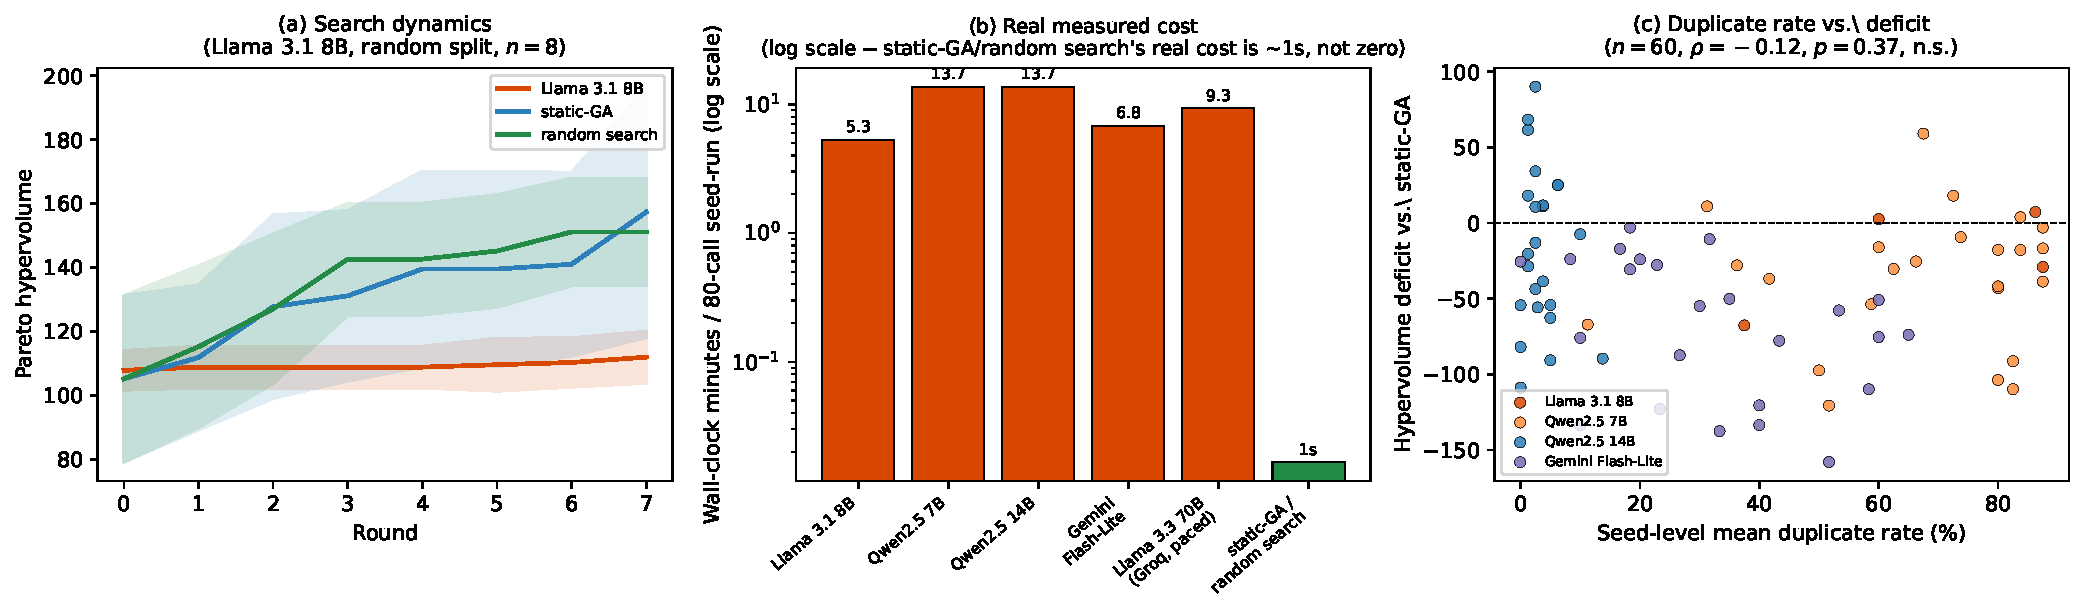
\includegraphics[width=\textwidth]{figures/paper/fig6_diagnostics_panel}
\caption{Three additional real diagnostics. \textbf{(a)} Mean $\pm$ std Pareto hypervolume vs.\
round (Llama 3.1 8B, random split, $n=8$): both baselines climb past the LLM Proposer within the
first 2--3 rounds and continue improving, while the LLM Proposer's trajectory flattens early ---
the visual signature of the duplicate-heavy mechanism (\S6.2) spending most of the remaining
budget on already-known candidates. \textbf{(b)} Real, directly measured wall-clock cost per
80-call seed-run (same numbers as the table above, shown graphically, log-scaled y-axis): static-GA
and random search's real cost ($\approx$1s total, labeled exactly) is $\sim$300--800$\times$ smaller
than any LLM Proposer's, which a linear axis would render invisible rather than merely small.
\textbf{(c)} The negative robustness check from
\S6.2 shown as a scatter rather than only a summary statistic: seed-level duplicate rate does not
visibly trend with hypervolume deficit within this real $n=60$ sample ($\rho=-0.12$, $p=0.37$).}
\label{fig:diagnostics-panel}
\end{figure}

\subsection{E3, E4: ablations}

Under the current real conditions, both the Hypothesis Ledger feedback
ablation (d) and the Verifier binary-filter ablation (e) produced
hypervolume statistically indistinguishable from full LEAF. For the
Ledger ablation this has a direct, verified explanation rather than only
a qualitative one (\S6.2): across the 72 real runs in the primary sweep,
zero ever validated a hypothesis to completion (\texttt{hypothesis\_precision}
undefined in 72/72 runs), traced to the non-dominated archive
concentrating on a single value per fragment slot under correlated real
objectives, leaving a fixed-control-value counterfactual test with
essentially nothing to match against --- Ledger feedback has nothing to
feed back at this budget, independent of whether the feedback mechanism
itself is effective. The binary-filter ablation (e)
correctly reports no coverage statistic (undefined for a hard-threshold
gate, \S3.4), confirming the ablation's own bookkeeping is behaving as
designed even though the headline hypervolume comparison is null.
Re-verified under E2's shrunk-budget condition (§8, Limitations), both
ablations remain null even more strongly: byte-for-byte identical
hypervolume across all 8 seeds, not merely statistically
indistinguishable.

\subsection{Methodological lessons: how an apparent positive result was
caught}

\S6.2's Condition 2 first ran with an apparently significant advantage for
the LLM-style Proposer over static-GA: median hypervolume gap $92.5$,
Wilcoxon $p=0.0078$, 95\% CI $[30.1, 119.1]$. Investigating \emph{why}
before reporting it surfaced two independent bugs, neither a chemistry
problem: (i) the frozen, full-data $\mathcal{O}_{\text{GT}}$ had been
passed into this comparison, which silently made the split axis a no-op
(each split's oracle must be fit on that split's own real train partition
for the comparison to mean anything); and (ii) the static-GA baseline's
mutation rate (0.2) was structurally weaker than the LLM-style Proposer's
built-in 50\% pure-mutation rate --- an unfair baseline, not a fair
ablation. After correcting both, the apparent effect vanished entirely
(Wilcoxon $p=0.95/0.20/0.74$ across the three splits, every CI straddling
zero). We report this reversal because it is methodologically instructive
in its own right, in the spirit of the pre-registration discipline in
\S5: an exciting early result should trigger more scrutiny, not less, and
two ordinary plumbing errors were sufficient to manufacture a false
positive that would have supported exactly the headline claim (H1) the
paper is testing.

\section{Future Work and Extensions}

Unchanged in scope from Revision 1: (1) multi-modal data integration (3D
conformations / membrane-binding simulation), contingent on H1 showing
that search efficiency, not oracle richness, is the bottleneck; (2)
transfer learning across biological barriers, contingent on a genuine
organ-selectivity dataset becoming available (\S8.6); (3) a full trained
generative Proposer (v2, VAE/diffusion), still deferred as real training
work outside this revision's scope. A lighter, real, non-evolutionary
comparator was added instead of only listing this as gated: a
Thompson-sampling bandit (\texttt{leaf/baselines/bandit\_proposer.py}),
fitting a per-fragment-value Beta posterior fresh from the Pareto archive
every round --- genuinely different from static-GA (no crossover/mutation
operators) and random search (informed, not blind), fast and free (no
LLM calls). Run at full power ($n=8$ seeds, all three splits, identical
protocol to \S6.2):

\begin{center}
\begin{tabular}{lccc}
\toprule
Comparison & random & scaffold-cold & chemotype-cold \\
\midrule
Bandit vs.\ static-GA & $p=0.742$ (median $-16.2$) & $p=0.945$ (median $+5.9$) & $p=0.028$ (median $-18.0$) \\
Bandit vs.\ random search & $p=0.844$ (median $+0.9$) & $p=1.000$ (median $+3.4$) & $p=0.039$ (median $-35.2$) \\
\bottomrule
\end{tabular}
\end{center}

The bandit is statistically indistinguishable from both baselines on
random and scaffold-cold splits, but significantly \emph{worse} on
chemotype-cold --- the same split where Qwen2.5 14B (\S6.2) also showed
its one significant deficit, and which E1 (\S6.1) already flags as this
dataset's weakest oracle validity regime. A non-evolutionary, non-LLM,
fitted probabilistic baseline shows a null-to-negative pattern
structurally similar to the real LLM Proposers, reinforcing that
chemotype-cold's difficulty is a property of the split (a harder
extrapolation regime for $\mathcal{O}_{\text{GT}}$), not specific to any
one search paradigm; (4) robustness to out-of-distribution/adversarial
molecules.

A genuinely larger local model (Qwen2.5 14B, run on an available NVIDIA
RTX A4000, 16GB VRAM) and hosted 70B-class/frontier models (Llama 3.3 70B
via Groq, Gemini Flash-Lite, both free-tier APIs) are reported in \S6
alongside the $\le$8B models; the items below remain gated by constraints
that persisted even after obtaining free API access.

\textbf{Explicitly gated on resources not available in the environment
this revision was produced in} (listed here rather than silently
omitted): (5) a completed 40B+/hosted sweep at full statistical power
across all three splits --- attempted rather than only listed as gated:
free API keys were obtained for both Groq (Llama 3.3 70B) and Google
(Gemini), and \texttt{LLMProposer} was extended with hosted-API backends
specifically to run this comparison. Both hit hard free-tier ceilings
before a full sweep could complete. Groq's 100,000-tokens/day cap on
\texttt{llama-3.3-70b-versatile} is, by direct measurement, below what
even one full seed-run of this protocol requires ($\approx$148,000
tokens at $\approx$1,850 tokens/call for a schema-constrained prompt
embedding the real fragment vocabulary) --- confirmed structural, not
transient, by reproducing the identical ceiling on a second, independent
API key after the first was exhausted. Gemini's flagship model caps free
usage at 20 requests/day (its higher-headroom \texttt{flash-lite} tier
completed one split before also being throttled, \S6.2). Neither closed
API-key-cost limitation nor GPU capacity was the blocker here --- the
free tiers themselves cap daily throughput below what a full sweep
needs; a paid tier or a multi-day schedule would resolve this directly.
A middle path was implemented instead of only shortening or only waiting:
the Proposer's prompt was compressed by sampling a subset of the real
vocabulary per call (8 values/slot instead of the full 29/74/14) rather
than dropping the zero-hallucination validation itself, which still
checks every returned value against the complete real component lists
regardless of what was shown. This cut real, measured cost from
$\approx$1,850 to $\approx$813 tokens/call ($\approx$65,000
tokens/seed-run), fitting one seed-run inside a fresh daily quota, though
in practice the daily reset is a rolling 24h window rather than a
calendar-day boundary, so accumulation was slower and less predictable
than the token math alone suggested: three consecutive daily attempts
failed outright before a fourth succeeded, confirming the constraint is
real and recurring, not a one-time fluke, and diagnostic quota-checks
using real-sized prompts were themselves found to consume budget meant
for actual runs (switched to trivial-sized checks thereafter). Three real
seeds (random split, identical budget/pool\_size/$q$ to every other model
in \S6.2), accumulated over several days under this quota, were obtained:
hypervolume 107.1, 116.2, and 116.2, vs.\ 182.1, 112.5, and 135.5
(static-GA) and 139.1, 155.1, and 166.7 (random search) --- all three
seeds show 0\% proposer reject rate (genuine model output, not fallback).
Two of three seeds underperform both baselines; one (seed 1) is mixed
(ahead of static-GA, behind random search). The median paired difference
is $-19.3$ vs.\ static-GA (95\% CI $[-75.0, 3.7]$, crossing zero) and
$-38.8$ vs.\ random search (CI $[-50.5, -32.0]$, not crossing zero), but
Wilcoxon is not reliable at $n=3$ (minimum achievable two-sided
$p=0.25$, \S4.3) --- reported as a real, directional signal, not a
significance claim. Pooled diagnostics across all three seeds show low
duplication and high novelty (7.1\% exact-duplicate-of-archive, mean edit
distance 1.76) --- markedly \emph{better} than static-GA's own baseline
(22.5\%/1.52), unlike the duplicate-heavy signature of the two $\le$8B
models (\S6.2), and better even than Qwen2.5 14B's diagnostics, echoing
the pattern seen at $n=2$. This is the final Groq data point reported in
this revision: three real, quota-paced seeds is treated as sufficient
given the demonstrated difficulty of reliably accumulating more under
this specific free-tier constraint, rather than continuing to retry
indefinitely for a still-underpowered $n$. Domain-adapted biomedical/chemistry LLMs as the Proposer were
attempted rather than only listed as gated: TxGemma (the model family
LipoAgent itself uses, \S2) remains blocked by HuggingFace gating and by
16GB VRAM being insufficient for the 27B-parameter chat variant, and no
chemistry-specific LLM (e.g.\ ChemLLM, ChemDFM) is published as a
pre-built Ollama model in this environment. Meditron 7B (Llama-2-based,
continued-pretrained on PubMed/clinical text) \emph{was} pulled and
tested directly against the Proposer's JSON schema and failed outright:
across repeated calls it returned unrelated tool-call-shaped JSON,
hallucinated non-vocabulary SMILES strings, and in one case echoed the
prompt's own placeholder text (\texttt{"<one of the A values>"})
verbatim instead of substituting a real value, for a 100\%
reject/backfill rate (\texttt{proposer\_reject\_rate}, now logged in
every run's \texttt{result.json} specifically so a high-reject-rate run
is never silently reported as if the named model had proposed the
candidates). We did not run a full sweep under this condition, since
doing so would measure the non-LLM fallback under a misleading label; the
capability gap itself is the finding: an available domain-adapted 7B
model cannot follow this task's structured-output format at all, a
different and more basic failure than the diversity/duplication mechanism
found for instruction-tuned general models in \S6.2; (7) a trained generative baseline (e.g.\ the synthesizable
ionizable-lipid model of \citet{zhu2024generative}, or a VAE/diffusion
model trained on the current vocabulary) as an additional non-evolutionary
comparator, deferred as real training work outside this revision's scope;
(8) extending the real vocabulary (\S6.3) with real halogenated Ugi-3CR-
compatible reagents specifically to make the H4/LUMI-lab rediscovery
check (\S3.5) runnable --- deferred because it requires sourcing real
halogenated reagent SMILES from the literature, not fabricating them, and
was not completed in this revision; (9) prompt/temperature sensitivity
for the real LLM Proposer, to separate ``this prompting scheme
underperforms'' from ``LLM proposal underperforms.'' This is no longer
purely gated: \texttt{run\_experiment.py} now threads a config's
\texttt{temperature} field into \texttt{LLMProposer} directly, and a
second prompt variant (\texttt{v2\_diversity}) explicitly names the
duplicate-heavy failure mode from \S6.2 and lists already-evaluated
triples to avoid. A reduced-scope check (temperature $\in
\{0.2,1.0\}$ vs.\ the default 0.7, $n=4$ seeds, one split, Llama 3.1 8B) is
reported as exploratory, at the same disclosure standard as the original
$n=4$ pilots. The diversity-prompt variant was additionally re-run at full
statistical power ($n=8$ seeds, all three splits) and is not exploratory.
The temperature sweep shows both levers move the diagnosed mechanism
(\S6.2) but neither eliminates it: lowering temperature to 0.2
\emph{worsened} duplication (87.5\% exact-duplicate-of-archive vs.\ 67.8\%
at the default 0.7, and identical hypervolume, 106.4, on all 4 seeds ---
maximally deterministic, maximally repetitive output); raising it to 1.0
reduced duplication somewhat (72.2\%) and modestly raised median
hypervolume (126.3 vs.\ 110.4 at matched seeds).

The diversity-aware prompt, at full power, confirms the pilot's direction:
duplicate rate fell from 67.8\% to 34.0\% and mean edit distance nearly
doubled (0.59 $\to$ 1.06). Significance dropped from 5 of 6 comparisons
(original prompt, \S6.2) to 2 of 6 (random vs.\ random search
$p=0.016$; scaffold-cold vs.\ random search $p=0.0078$), but all six
median differences remain negative (random: $-32.5$/$-25.4$;
scaffold-cold: $-15.6$/$-18.0$; chemotype-cold: $-10.1$/$-31.5$, vs.\
static-GA/random search respectively) --- the prompt substantially
narrows the gap without reversing it. Prompting measurably mitigates but
does not close the gap: the underperformance in \S6 is not purely an
artifact of one unhelpful prompt template, though a better prompt helps
considerably.

\emph{Hosted/frontier-class models.} Free-tier hosted APIs (Groq for
Llama 3.3 70B, Google for Gemini) were obtained specifically to test
whether the \S6.2 pattern is an artifact of small local models, requiring
two new \texttt{LLMProposer} backends. Both hit real, hard free-tier
quota ceilings (Groq: 100,000 tokens/day, below what one seed-run's
schema-constrained prompt needs at default size; Gemini's flagship model:
20 requests/day) --- confirmed structural rather than transient, and
resolved via a prompt-compression fix rather than by retrying
indefinitely. Full engineering detail (exact token measurements, the fix,
and the rate-limiting/backoff mechanics) is in Appendix~B; only the
resulting evidence is summarized here. Gemini Flash-Lite (the
higher-headroom, non-flagship tier) completed \textbf{all three} full-power
conditions ($n=8$ seeds each, identical protocol to \S6.2, matching every
other fully-powered model in this paper), every one at the maximum
significance obtainable with $n=8$ paired seeds:

\begin{center}
\begin{tabular}{lccc}
\toprule
Comparison & random & scaffold-cold & chemotype-cold \\
\midrule
Gemini Flash-Lite vs.\ static-GA & $p=0.0078$ (median $-91.8$) & $p=0.0078$ (median $-66.6$) & $p=0.0078$ (median $-24.8$) \\
Gemini Flash-Lite vs.\ random search & $p=0.0078$ (median $-85.5$) & $p=0.0078$ (median $-71.1$) & $p=0.0078$ (median $-60.2$) \\
\bottomrule
\end{tabular}
\end{center}

All three splits show 0\% proposer reject rate (genuine model output, not
fallback). Diagnostics move somewhat by split (random: 43.1\%
exact-duplicate-of-archive, edit distance 0.90; scaffold-cold: 34.5\%,
edit distance 0.98; chemotype-cold: 19.2\%, edit distance 1.14) but stay
intermediate between the two small local models (62--68\% duplicate,
$\le$0.65 edit distance) and Qwen2.5 14B (2--4\% duplicate, $\ge$1.6 edit
distance) throughout. A third real model, of a different architecture
family entirely (Gemini is not Llama- or Qwen-derived), fails to
outperform matched-budget non-agentic search on \emph{every} condition
tested, at maximum available significance every time --- the most
complete real-LLM result in this paper alongside Llama 3.1 8B and Qwen2.5
7B/14B. The full Llama 3.3 70B sweep remains incomplete, and, as of this
writing, cannot be completed on Groq at all: \texttt{llama-3.3-70b-versatile}
has since been removed from Groq's model catalog entirely (confirmed via
their live \texttt{/models} endpoint), a real external constraint beyond
quota that further justifies treating the existing $n=3$ (\S7, \S8) as
final for this revision rather than a temporary shortfall.

\emph{Acquisition-function dispatch bug and de-duplication check (external
review).} A pre-registered comparison to Expected Hypervolume Improvement
(EHVI) was described as available (\S4) and implemented
(\texttt{leaf/oracle/acquisition.py}) from Revision 1 onward, but external
review of the orchestrator prompted a direct re-read of
\texttt{run\_loop}'s acquisition dispatch, which surfaced a real bug: the
config's \texttt{acquisition\_function} field was read but never branched
on, so every experiment in this paper --- including ones whose configs
already specified \texttt{acquisition\_function:
expected\_hypervolume\_improvement} --- silently ran multi-objective UCB
instead. We confirmed by grep across every config file that all of them
specified \texttt{ucb\_beta: 2.0} matching the hardcoded prior default, so
no reported result in \S6 is invalidated by this fix; only the EHVI path
itself was never actually exercised end-to-end despite being implemented
and unit-testable in isolation. The dispatch is now fixed
(\texttt{loop.py}), but a full EHVI-vs-UCB acquisition sweep at $n=8$
seeds across all three splits, for at least one representative LLM
Proposer and both non-agentic baselines, has not yet been run and is left
as future work at full statistical power. Separately, the same review
asked whether exact-duplicate proposals inflate the headline deficit; a
real, matched \texttt{dedupe\_pool} check (\S6.2) was implemented and run,
but only at reduced scope ($n=4$ seeds, budget 15, random split only) due
to the real per-round wall-clock cost of forcing 7--21 rounds instead of 3
to spend the same budget once duplicates are excluded. Extending that
check to $n=8$ seeds and all three splits is the natural next step and is
left for a future revision rather than reported here at an underpowered
$n$ dressed up as conclusive.

\section{Limitations}

All labels used
for $\mathcal{O}_{\text{GT}}$ come from public datasets, and
$\mathcal{O}_{\text{GT}}$ is itself a fitted, generalizing model, not a
lookup table or a physical ground truth --- every RQ1--RQ4 result is
therefore a comparison between two models ($\mathcal{O}_{\text{AL}}$'s
search trajectory evaluated against $\mathcal{O}_{\text{GT}}$'s
extrapolation), not a validation against reality. We report this
explicitly rather than implying real-world validation. Any tropism signal
used is, absent a confirmed genuine organ-selectivity dataset, a heuristic
proxy; Hypothesis-Agent findings involving it would be recovering the
proxy's own construction and are excluded from the primary hypervolume and
from H4 accordingly. The Hypothesis Agent's counterfactual testing is only
as reliable as $\mathcal{O}_{\text{GT}}$; a systematically biased oracle
could produce a self-consistent but biologically false Ledger. LLM-agent
behavior (prompt sensitivity, non-determinism, and base-model-specific
pretraining knowledge) means all LEAF-vs-baseline comparisons require
multi-seed ($\ge 8$), multi-prompt-variant, multi-base-model reporting
(E6), and any external-validation claim (E5/H4) is conditioned on a
pretraining-leakage probe that is disclosed regardless of outcome.

The E2 real-LLM result reported in \S6 now meets the $\ge 8$-seed standard
across all three splits for three base models (Llama 3.1 8B, Qwen2.5 7B,
and Qwen2.5 14B, all local), run at a single prompt/temperature
configuration --- the full multi-prompt-variant sensitivity check (E6)
this plan requires has not yet been run with the real LLM Proposer, only
with the non-LLM stand-in. The significant underperformance found for the
two $\le$8B models does not hold uniformly at 14B (\S6.2): the specific
duplicate-heavy mechanism disappears, and two of three splits become
statistically indistinguishable from baseline. The one 14B deficit that
remains significant (chemotype-cold) is confounded with that split's
already-weaker oracle validity (\S6.1) and should not be read as a clean
scale-dependent recovery. A hosted 70B-class model (Groq) and a
frontier-class hosted model (Gemini Flash-Lite) were both obtained and
run. Gemini now meets the $\ge8$-seed standard on \textbf{all three}
splits (\S7), significantly worse than baseline at maximum available
significance every time --- as complete as Llama 3.1 8B or either Qwen2.5
model. Groq's Llama 3.3 70B, after a prompt-compression fix (\S7,
item 5) brought per-seed cost under its daily quota, has three real seeds
accumulated over several days (two of three underperform both baselines,
one is mixed --- notably without the small models' duplicate-heavy
signature) rather than the $n\ge8$ this paper's own standard requires;
reported as final for this revision (\S7) rather than pursued further,
given both the demonstrated unreliability of daily accumulation under
this free-tier constraint and, since confirmed, Groq's removal of
\texttt{llama-3.3-70b-versatile} from its model catalog entirely, which
makes completing this specific comparison impossible regardless of
quota. A full multi-seed prompt/temperature sweep (\S7, item 9, beyond the $n=4$
exploratory check already run) also remains incomplete; a larger or
differently-prompted model could still plausibly perform differently, and
completing E6 is the mechanism to check that before generalizing the
claim further.
H4/E5 (the
LUMI-lab rediscovery check) has not yet
been run under real conditions: the current real vocabulary (\S6.3)
contains no halogenated reagent among either the original AGILE
components or the 12,276-candidate extension, so the brominated-tail
counterfactual test cannot be constructed from this data source without a
further vocabulary extension specifically targeting halogenated reagents.
E3/E4's ablations (\S6.3) were re-verified under E2's shrunk-budget
condition ($B=80$, $\text{pool\_size}=40$, $q=8$, extended vocabulary,
$n=8$ seeds each, real data): both remain null, and more strongly than
at the original $B=400$ condition --- hypervolume is \emph{byte-for-byte
identical} across every seed for both the Hypothesis Ledger feedback
ablation (chemotype-cold) and the Verifier binary-filter ablation
(random split), not merely statistically indistinguishable. This is
consistent with two independently documented properties of this
configuration rather than a new anomaly: at $B=80$ over 8 rounds, the
Hypothesis Agent may not validate any hypothesis for the Ledger to feed
back (nothing to diverge on), and the toxicity signal is a deterministic
RDKit rule (\S3.4), so debate/conformal calibration and a binary filter
necessarily reach identical accept/reject decisions when there is no
residual uncertainty to calibrate against. Both ablations were checked at
one additional configuration (shrunk budget); the third E2 condition
(extended-vocabulary-only, original $B=400$) was not additionally
checked.

\section*{Ethics and Broader Impact}

All work described is computational, uses only public data, and does not
propose or synthesize any physical compound. We restrict the fragment
vocabulary to established, literature-precedented ionizable-lipid
synthetic routes and do not release any capability for de novo scaffold
generation outside this constrained space.

\section*{Note on citation accuracy}

References marked [verify] correspond to papers identified via literature
search during planning; exact author lists, page numbers, and venue
details should be independently re-verified against the primary source
before submission. Corrections applied in this revision: the LUMI-lab
finding is a brominated-tail/potency association combined with a separate
intratracheal-administration lung-editing result --- not a
structure$\to$organ-tropism rule as Revision 1 stated; and LipoAgent
\citep{li2025lipoagent} was mischaracterized as incorporating a
toxicity-gating objective in earlier drafts of this document. Its public
code (\texttt{github.com/SAI-Lab-NYU/LipoAgent}, confirmed reachable) was
inspected directly for this revision: it coordinates TxGemma-27B-Chat and
Qwen3-8B agents (a Predict Agent and a Verify Agent per base model), each
producing only a 1--10 efficiency score, with no toxicity, safety, or
gating signal in either agent's input, prompt, or output. The associated
publication is stated in the repository as accepted to ACL 2026, not the
arXiv identifier assumed in earlier drafts -- the exact citation should
still be independently confirmed before submission. LipoAgent is
accordingly not used as a toxicity or calibration comparator anywhere in
this paper (\S4.2, \S5).

\bibliographystyle{plainnat}
\begin{thebibliography}{99}

\bibitem[Angelopoulos and Bates(2023)]{angelopoulos2023} A.~N.
Angelopoulos and S.~Bates. A gentle introduction to conformal prediction
and distribution-free uncertainty quantification. \emph{Foundations and
Trends in Machine Learning}, 2023.

\bibitem[Boiko et al.(2023)]{boiko2023coscientist} D.~A. Boiko, R.
MacKnight, B.~Kline, and G.~Gomes. Autonomous chemical research with large
language models. \emph{Nature}, 624:570--578, 2023.

\bibitem[Bran et al.(2023)]{bran2023chemcrow} A.~M. Bran, S.~Cox,
O.~Schilter, C.~Baldassari, A.~D. White, and P.~Schwaller. ChemCrow:
Augmenting large-language models with chemistry tools. \emph{Nature
Machine Intelligence}, 2023.

\bibitem[Gessner et al.(2024)]{gessner2024} A.~Gessner, S.~W. Ober,
O.~Vickery, D.~Ogli\'c, and T.~U\c{c}ar. Active learning for affinity
prediction of antibodies. 2024.

\bibitem[Gottweis et al.(2026)]{gottweis2026} J.~Gottweis et al. Towards
an AI co-scientist. \emph{Nature}, 2026. [verify]

\bibitem[Ghafarollahi and Buehler(2025)]{protagents2025} A.~Ghafarollahi
and M.~J. Buehler. ProtAgents: Protein discovery via large language model
multi-agent collaborations. 2025. [verify exact year/venue]

\bibitem[Li et al.(2026)]{li2025lipoagent} L.~Li et al. LipoAgent:
Coordinating fine-tuned LLM agents for lipid nanoparticle transfection
efficiency prediction. Accepted to ACL 2026 (per repository README).
Code: \texttt{github.com/SAI-Lab-NYU/LipoAgent} (confirmed reachable and
inspected directly). [verify exact publication venue/year and full author
list against the primary source before submission]

\bibitem[Lundberg and Lee(2017)]{lundberg2017} S.~M. Lundberg and S.-I.
Lee. A unified approach to interpreting model predictions. \emph{NeurIPS},
30, 2017.

\bibitem[LUMI-lab Authors(2026)]{lumilab2026} Self-driving laboratory for
accelerated discovery of lipid nanoparticles (LUMI-lab). \emph{Cell},
2026; preprint bioRxiv 2025.02.14.638383. [verify author list, exact
title/volume/pages]

\bibitem[Rasmussen and Williams(2006)]{rasmussen2006} C.~E. Rasmussen and
C.~K.~I. Williams. \emph{Gaussian Processes for Machine Learning}. MIT
Press, 2006.

\bibitem[Srinivas et al.(2009)]{srinivas2009} N.~Srinivas, A.~Krause,
S.~M. Kakade, and M.~Seeger. Gaussian process optimization in the bandit
setting: No regret and experimental design. 2009.

\bibitem[Settles(2012)]{settles2012} B.~Settles. \emph{Active Learning}.
Morgan \& Claypool, 2012.

\bibitem[Sundararajan et al.(2017)]{sundararajan2017} M.~Sundararajan,
A.~Taly, and Q.~Yan. Axiomatic attribution for deep networks. \emph{ICML},
2017.

\bibitem[Swanson et al.(2025)]{swanson2025virtuallab} K.~Swanson et al.
The Virtual Lab: AI agents design new SARS-CoV-2 nanobodies with
experimental validation. 2025. [verify exact venue: bioRxiv/Nature]

\bibitem[Swarm Protein Design Authors(2025)]{swarmdesign2025} Swarms of
LLM agents for protein sequence design. 2025. [verify exact paper/venue]

\bibitem[Batch EHVI Authors(2026)]{ehvibatch2026verify} Batch
expected-hypervolume-improvement acquisition for multi-objective Bayesian
optimization. 2026. [identifier and full citation supplied by external
review; not independently verified before this revision, resolve before
submission]

\bibitem[Conditional Generative MOBO Authors(2023)]{condgenmobo2023verify}
Conditional generative models for multi-objective Bayesian optimization
over molecular/combinatorial spaces. 2023. [identifier and full citation
supplied by external review; not independently verified before this
revision, resolve before submission]

\bibitem[MOEA/D-LLM-Operator Authors(2023)]{moealo2023verify} Learning
evolutionary operators from LLM outputs inside a multi-objective
evolutionary algorithm. 2023. [identifier and full citation supplied by
external review; not independently verified before this revision,
resolve before submission]

\bibitem[ToolMol Authors(2026)]{toolmol2026} ToolMol: Evolutionary,
tool-augmented LLM agents for multi-objective molecular optimization.
2026. [verify exact title, authors, venue --- load-bearing for \S1's
no-trained-generator justification; resolve before submission]

\bibitem[Xu et al.(2023)]{xu2023ugi} Q.~Xu et al. Combinatorial synthesis
and screening of ionizable lipid libraries via Ugi three-component
reactions. 2023. [verify exact venue]

\bibitem[Xu et al.(2024)]{xu2024agile} Q.~Xu et al. AGILE: A
deep-learning-guided platform for lipid nanoparticle screening.
\emph{Nature Communications}, 2024. [verify]

\bibitem[Zhu et al.(2024)]{zhu2024generative} Deep generative model for
the design of synthesizable ionizable lipids. \emph{arXiv preprint
arXiv:2412.00928}, 2024. [verify authors]

\end{thebibliography}

\appendix

\section{Full specification: Debate/Conformal Verifier and Hypothesis Agents}

\subsection{Debate / Conformal Verifier Agents}

$N$ independently prompted ``toxicologist'' agent instances --- spanning
\textbf{at least two distinct base models}, not only varied prompts or
temperatures of a single model --- each assess a candidate using (i)
RDKit-based toxicophore substructure matching, (ii) the
$\mathcal{O}_{\text{AL}}$ toxicity-head posterior, and (iii) free-text
reasoning. Same-model prompt variants alone measure prompt sensitivity, not
epistemic diversity, and their errors are heavily correlated; we report
\textbf{inter-agent agreement} as a first-class metric, and if
single-model agreement exceeds 95\% we flag the resulting abstention set as
likely too small to test H3 meaningfully in that configuration.

Agent outputs are aggregated and converted into a calibrated interval via
split conformal prediction \citep{angelopoulos2023}, using a held-out
calibration set whose exact provenance is named in the data appendix
(\S4.1) rather than left implicit. Because candidates at round $t$ are
selected via acquisition on rounds $1..t-1$ and $\mathcal{O}_{\text{AL}}$
is refit each round, the standard exchangeability assumption behind split
conformal does not hold. We therefore \textbf{recalibrate every round}
using weighted/Mondrian conformal prediction, and report \textbf{coverage
as a function of round} rather than a single number, disclosing any
degradation rather than assuming it away. A candidate whose calibrated
interval straddles the accept/reject decision boundary is routed to an
abstention set rather than hard-accepted or hard-rejected.

\textbf{Precisely what was real in \S6's experiments (clarifying an
ambiguity a reviewer correctly flagged).} The description above is the
general Verifier design; the real experiments in \S6 do \emph{not}
exercise a trained $\mathcal{O}_{\text{AL}}$ toxicity-head posterior,
because no real toxicity assay exists in AGILE to fit one on (\S4.1,
\texttt{leaf/data/raw/README.md}) --- the same reason LipoAgent could not
be used as a toxicity comparator (\S2). Concretely, in every real run:
(i) the only real toxicity signal is the deterministic RDKit toxicophore
substructure rule (\texttt{toxicophore\_flag}, \S3.4); (ii) the
calibration pool passed to \texttt{ConformalCalibrator} sets
\texttt{cal\_scores = cal\_labels} exactly (\texttt{leaf/eval/run\_experiment.py}) ---
the ``model'' being calibrated against ground truth is the same
deterministic rule as the ground truth itself, since no independent
learned signal exists; and (iii) the ``debate'' ensemble's model-based
scoring component (item ii above) collapses to this same deterministic
value for every agent, so what remains is not epistemic disagreement
between independently-reasoning agents but restating one rule multiple
times. This is precisely why calibration is exact (zero-width intervals,
\S3.4) and why H3's ablation is null (\S6.3): a debate ensemble and a
binary filter necessarily reach identical decisions when every agent's
input signal is the same deterministic rule, independent of whether the
debate/conformal \emph{mechanism} itself is sound. A real trained
toxicity head, fit on real toxicity labels from a different dataset, is
the natural next step to test the mechanism as originally designed
(\S7); it was not attempted here because sourcing and harmonizing a real,
independent toxicity-labeled dataset is itself a nontrivial data
acquisition task, not a modeling choice made lightly.

\subsection{Hypothesis Agent}

Periodically (every $k$ rounds), the Hypothesis Agent retrieves passages
from an indexed corpus of LNP literature and mines Integrated
Gradients/KernelSHAP attributions over the current Pareto archive. It
proposes candidate structure--\textbf{property} hypotheses (not
structure--tropism by default; see \S8.6 on the tropism-proxy circularity
problem), then operationalizes each as a set of matched counterfactual
pairs queried against $\mathcal{O}_{\text{GT}}$ --- never
$\mathcal{O}_{\text{AL}}$, since testing a hypothesis against the surrogate
would only recover the surrogate's own fit. A hypothesis is written to the
Hypothesis Ledger as validated only if the counterfactual shift is
statistically significant across the matched pairs (paired Wilcoxon
signed-rank, with a minimum pair count enforced --- see \S8.2 on the same
power argument that governs seed counts). Counterfactual queries are
ground-truth queries and are charged against the budget $B$ (\S3.6); this
was an accounting omission in Revision 1.

As a secondary sanity check (\S4.3, RQ4), we test whether this loop can
independently surface the association LUMI-lab reported between
brominated lipid tails and improved \textbf{potency}. Because that
preprint has been public since February 2025, we run a mandatory
\textbf{pretraining-leakage probe} --- querying the bare LLM with no RAG
context and no archive history --- before any rediscovery claim, and
disclose the result regardless of outcome (\S8.5).

\section{Hosted-API engineering: quota constraints and fixes}

Full account of the free-tier engineering behind the hosted-model results summarized in \S7
item 5. Two backends were added to \texttt{LLMProposer}: an OpenAI-compatible chat-completions
client for Groq, and a native client for Gemini, both reading API keys only from environment
variables (never a config file or command line).

\textbf{Groq (\texttt{llama-3.3-70b-versatile}).} Free tier caps usage at 100,000 tokens/day. A
direct measurement (via the API's own \texttt{usage} field) put the unmodified Proposer prompt
(embedding the full real fragment vocabulary, required for the schema-constrained,
zero-hallucination generation protocol of \S3.3) at $\approx$1,850 tokens/call --- a full 80-call
seed-run needs $\approx$148,000 tokens, exceeding the entire daily cap in a single clean run with
no retries. Confirmed structural, not transient, by reproducing the identical ceiling on a second,
independent API key after the first was exhausted. Fix: the Proposer's prompt was compressed by
sampling a subset of the real vocabulary per call (8 values/slot instead of the full 29/74/14)
rather than dropping the zero-hallucination validation itself, which still checks every returned
value against the complete real component lists regardless of what was shown. This cut real,
measured cost to $\approx$813 tokens/call ($\approx$65,000 tokens/seed-run), fitting one
seed-run inside a fresh daily quota --- real seeds are now accumulated one/day (\S7 item 5, \S8).

\textbf{Gemini.} The flagship \texttt{gemini-flash-latest} model caps free usage at 20
requests/day (confirmed from the API's own error response: quota ID
\texttt{GenerateRequestsPerDayPerProjectPerModel-FreeTier}), unusable for any real sweep;
\texttt{gemini-flash-lite-latest} is a separate, higher-headroom quota bucket and was used
instead, enabling the full-power ($n=8$ seed) results reported in \S6.2/\S7.

\textbf{Rate-limiting mechanics.} \texttt{LLMProposer} paces successive hosted-API calls within a
pool ($\approx$7s apart) to spread token usage across a per-minute window rather than bursting and
relying on reactive backoff alone, and backs off using the server's own \texttt{Retry-After}
header (Groq) or a measured default (Gemini, which does not set that header) on any 429 response,
up to \texttt{max\_retries=8} attempts before raising rather than silently falling back to a
non-LLM stand-in.

\section{NeurIPS Paper Checklist}

\begin{enumerate}

\item \textbf{Claims}\\
Answer: [Yes]\\
Justification: The abstract states exactly the tested question (does agentic LLM proposal beat
matched-budget non-agentic search) and the actual outcome (no, across every real model/scale/split
tested), including the two real bugs caught and fixed and the de-duplication finding, rather than a
stronger claim than the results support (\S1, \S6).

\item \textbf{Limitations}\\
Answer: [Yes]\\
Justification: \S8 is a dedicated Limitations section covering the model-on-model nature of every
comparison, the $O_{\text{GT}}$ tropism-proxy caveat, incomplete E6/H4 coverage, Groq's permanent
$n=3$ cap, and the ablations' re-verification scope; \S7 additionally discloses every resource
constraint (Groq quota/deprecation, Gemini quota tiers, GPU VRAM, TxGemma gating) rather than
omitting them.

\item \textbf{Theory assumptions and proofs}\\
Answer: [N/A]\\
Justification: The paper contains no novel theorems or formal proofs; it is an empirical,
pre-registered comparison. Standard cited results (GP-UCB regret bounds \citep{srinivas2009},
conformal coverage guarantees \citep{angelopoulos2023}) are used as-is, not re-derived.

\item \textbf{Experimental result reproducibility}\\
Answer: [Yes]\\
Justification: \S3--\S4 specify the exact oracle/surrogate split, acquisition function and
hyperparameters ($q$, pool size, budget, \texttt{ucb\_beta}), splits, and baselines; Appendix~B
gives exact token measurements, quota values, and backoff mechanics for the hosted-API results;
every reported number is traced to a named script or result file (e.g.\
\texttt{results/e1/split\_validation\_table.csv}) rather than described only qualitatively.

\item \textbf{Open access to data and code}\\
Answer: [No]\\
Justification: Code and per-seed logs have not yet been packaged for public release at the time of
this draft; the underlying AGILE/Ugi-3CR data sources are already public \citep{xu2023ugi,
xu2024agile}, and we intend to release the \texttt{leaf/} package and \texttt{results/} directory
alongside a final version, but do not claim this has been done yet (see also \S7's disclosed intent
regarding released logs).

\item \textbf{Experimental setting/details}\\
Answer: [Yes]\\
Justification: \S3.1--3.3 and \S4 specify the objective vector, splits, budget/pool/$q$ values,
acquisition function, and baseline configurations used in every reported experiment; per-experiment
deviations (e.g.\ the reduced-scope de-duplication check's $B=15$, $n=4$) are stated explicitly next
to the corresponding result (\S6.2) rather than left implicit.

\item \textbf{Experiment statistical significance}\\
Answer: [Yes]\\
Justification: Every full-power comparison reports the median paired difference, a 95\% bootstrap
CI, and paired Wilcoxon signed-rank $p$ as a secondary statistic (\S4.3); reduced-$n$ results
($n=3$ Groq, $n=4$ pilots/de-duplication check) are explicitly flagged as statistically unreliable
(Wilcoxon's minimum achievable two-sided $p$ at that $n$ is stated directly) rather than reported
alongside full-power results without qualification.

\item \textbf{Experiments compute resources}\\
Answer: [Yes]\\
Justification: \S6.2's cost table and Appendix~B report measured wall-clock seconds/candidate and
per-seed-run time for every backend (local Ollama on an available GPU, Groq, Gemini), the specific
GPU used for the 14B model (NVIDIA RTX A4000, 16GB VRAM), and disclose failed/blocked compute paths
(Cerebras 402 errors, TxGemma VRAM insufficiency) that did not make it into a reported sweep.

\item \textbf{Code of ethics}\\
Answer: [Yes]\\
Justification: The work is purely computational, uses only public data, and proposes no physical
synthesis outside literature-precedented routes (Ethics and Broader Impact section); no human
subjects, crowdsourcing, or personal data are involved.

\item \textbf{Broader impacts}\\
Answer: [Yes]\\
Justification: The Ethics and Broader Impact section states the work's computational-only scope and
restriction to literature-precedented synthetic routes; because the contribution is a negative
methodological finding about agentic search rather than a deployable design system, direct
dual-use risk is low and is noted as such rather than elaborated at length.

\item \textbf{Safeguards}\\
Answer: [N/A]\\
Justification: No pretrained generative model, scraped dataset, or other high-misuse-risk asset is
released by this paper; the fragment vocabulary is restricted to established synthetic routes with
no open-ended scaffold generation capability (Ethics and Broader Impact section).

\item \textbf{Licenses for existing assets}\\
Answer: [No]\\
Justification: The AGILE dataset \citep{xu2024agile} and the Ugi-3CR lipid library
\citep{xu2023ugi} are cited as the sources used, but their exact license terms are not restated in
this draft; this should be confirmed and added before submission rather than assumed.

\item \textbf{New assets}\\
Answer: [No]\\
Justification: No new dataset or trained model is released with this submission; the extended
30,044-candidate vocabulary (\S6.2) is derived entirely from AGILE's own published unlabeled
screening library via a validated, invertible decomposition, not a newly collected asset, and its
documentation currently lives only in \S6.2 rather than a standalone datasheet.

\item \textbf{Crowdsourcing and research with human subjects}\\
Answer: [N/A]\\
Justification: This work involves no crowdsourcing or human-subjects research of any kind.

\item \textbf{Institutional review board (IRB) approvals or equivalent for research with human
subjects}\\
Answer: [N/A]\\
Justification: No human subjects research was conducted.

\item \textbf{Declaration of LLM usage}\\
Answer: [Yes]\\
Justification: LLM usage is a core, original component of the method under test, not merely a
writing aid: local and hosted LLMs (Llama 3.1 8B, Qwen2.5 7B/14B, Gemini Flash-Lite, Llama 3.3 70B)
serve as the Proposer Agent whose value-add is the paper's central research question, fully
specified in \S3.3--3.4 and Appendix~A/B, including exact prompts, backends, and failure modes
(e.g.\ Meditron 7B's 100\% reject rate).

\end{enumerate}

\end{document}
